\section{Results, Evaluation and Experiments}
In this section, we will discuss the results obtained in multiple conditions. Those data were recorded using ROSBag and were parsed using the ROSBag python module.
ROSbag is a program included with RORS, it is used to store and replay the messages published on ROS topics by ROS node.
We provide a jupyter notebook in the repository that facilitates drawing all the relevant graphs with a convenient way of storing all the parsed bags inside a pickle file.

\subsection{Compensation for drag}
In the first experiment, we will justify the need for an air drag compensation term. 
The velocity field we use in the circular velocity field is based on \cite{mcinnes2003velocity}.
\subsubsection{Experience without drag compensation}
\begin{figure*}[h!]
   \centering
   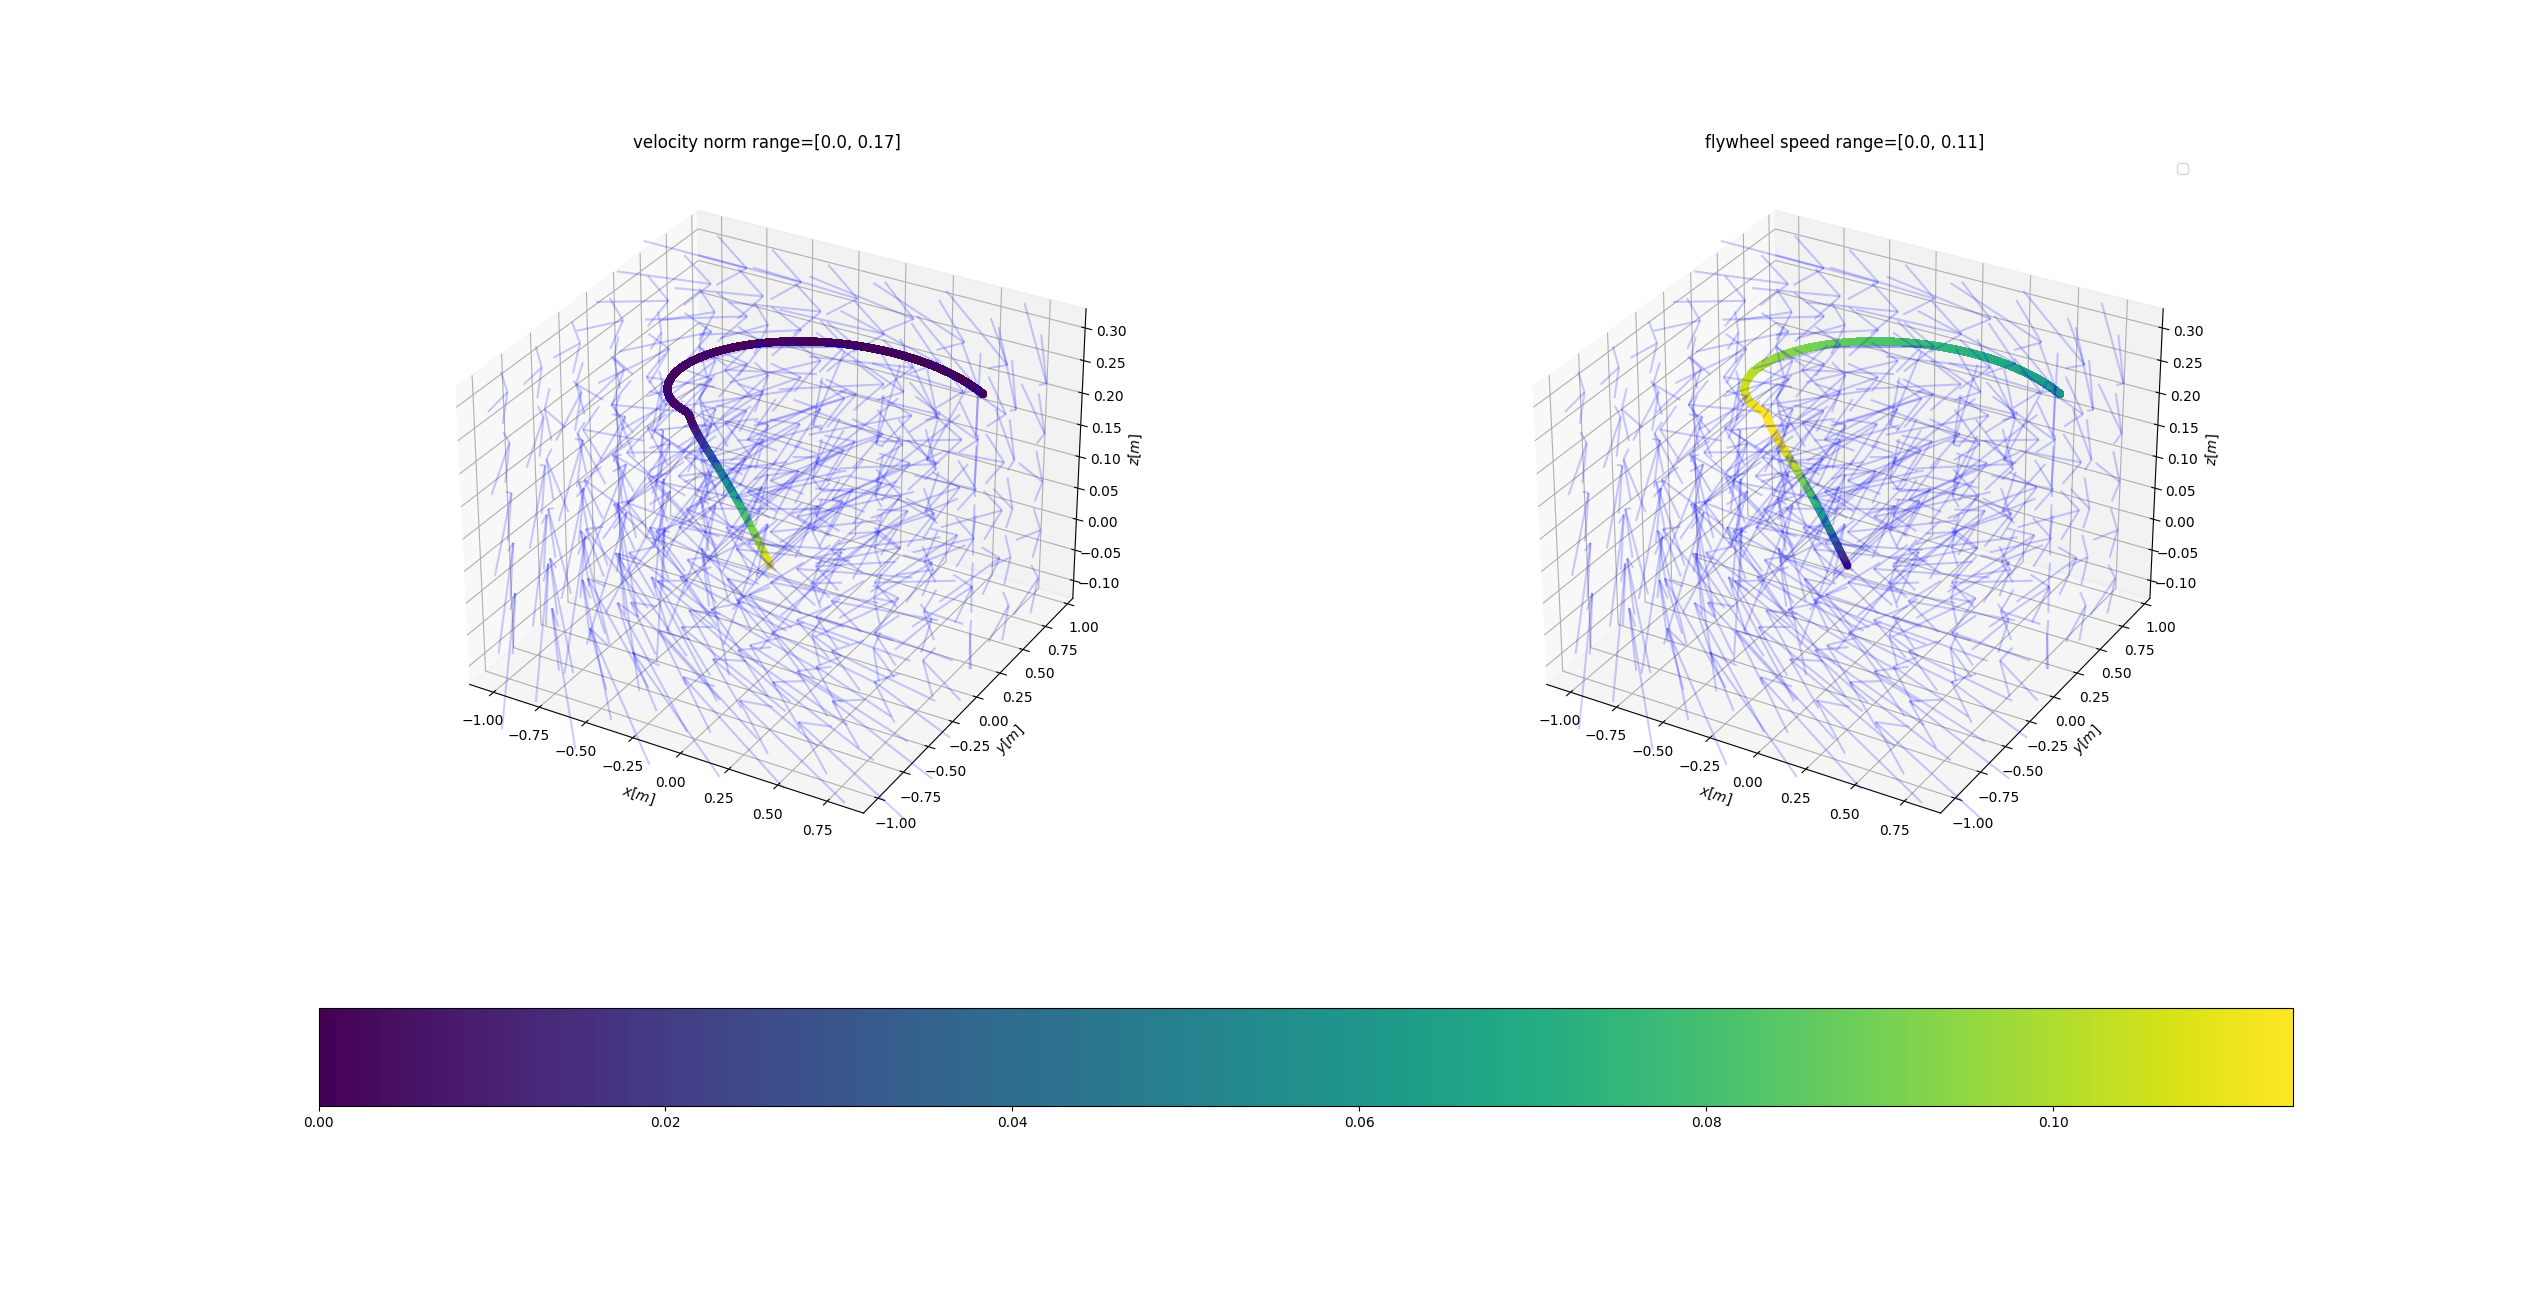
\includegraphics[width=\linewidth]{Images/python-noforcecomp.png}
   \caption{trajectory and mechanical energy without force compensation }
   \label{fig:pythonnocomp}
\end{figure*}
On the both of figure \ref{fig:pythonnocomp}, we can see the trajectory of the quadcopter, the left scatter plot of the trajectory is colored according to the
translational velocity of the quadcopter while the right scatter plot is colored according to the angular velocity of the fictitious flywheel.
On both subplots, the quiver plot represents the desired velocity field.
We can see that when we do not introduce a drag force compensation, the quad translational velocity goes to zero. 
This is explained by the fact by the quadcopter thrust given by PVFC has a too low amplitude to compensate the drag force and consequently the quad decelerates.
The amplitude of the flywheel velocity is not affected by this drag because we defined a perfect no friction flywheel.\\
These subplots are useful to observe how energy is being transfered between the fictitious flywheel and the quadcopter. 
We can see that as expected from equation \ref{eqn:vfly}, the faster the quad is going the slower the fictitious flywheel is spinning.

\begin{figure}[h!]
   \centering
   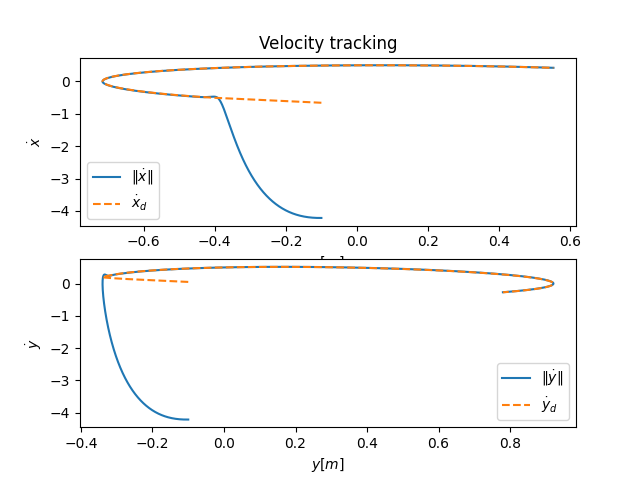
\includegraphics[width=\linewidth]{Images/velocitytrackingpythonnocomp.png}
   \caption{Trajectory tracking without force compensation }
   \label{fig:trajtracknocomp}
\end{figure}

Despite the total stop, we can see from the figure \ref{fig:trajtracknocomp} that the field is accurately followed.
\subsubsection{Experience with drag compensation}
This experiment is the same as the last one except that we add to the desired PVFC thrust output the compensation term $\tau_{comp} = C\cdot \dot{q}$ 
where $C$ is current translational coriolis matrix and $\dot{q}$ is the current translational velocity of the quadcopter.
\begin{figure*}[h!]
   \centering
   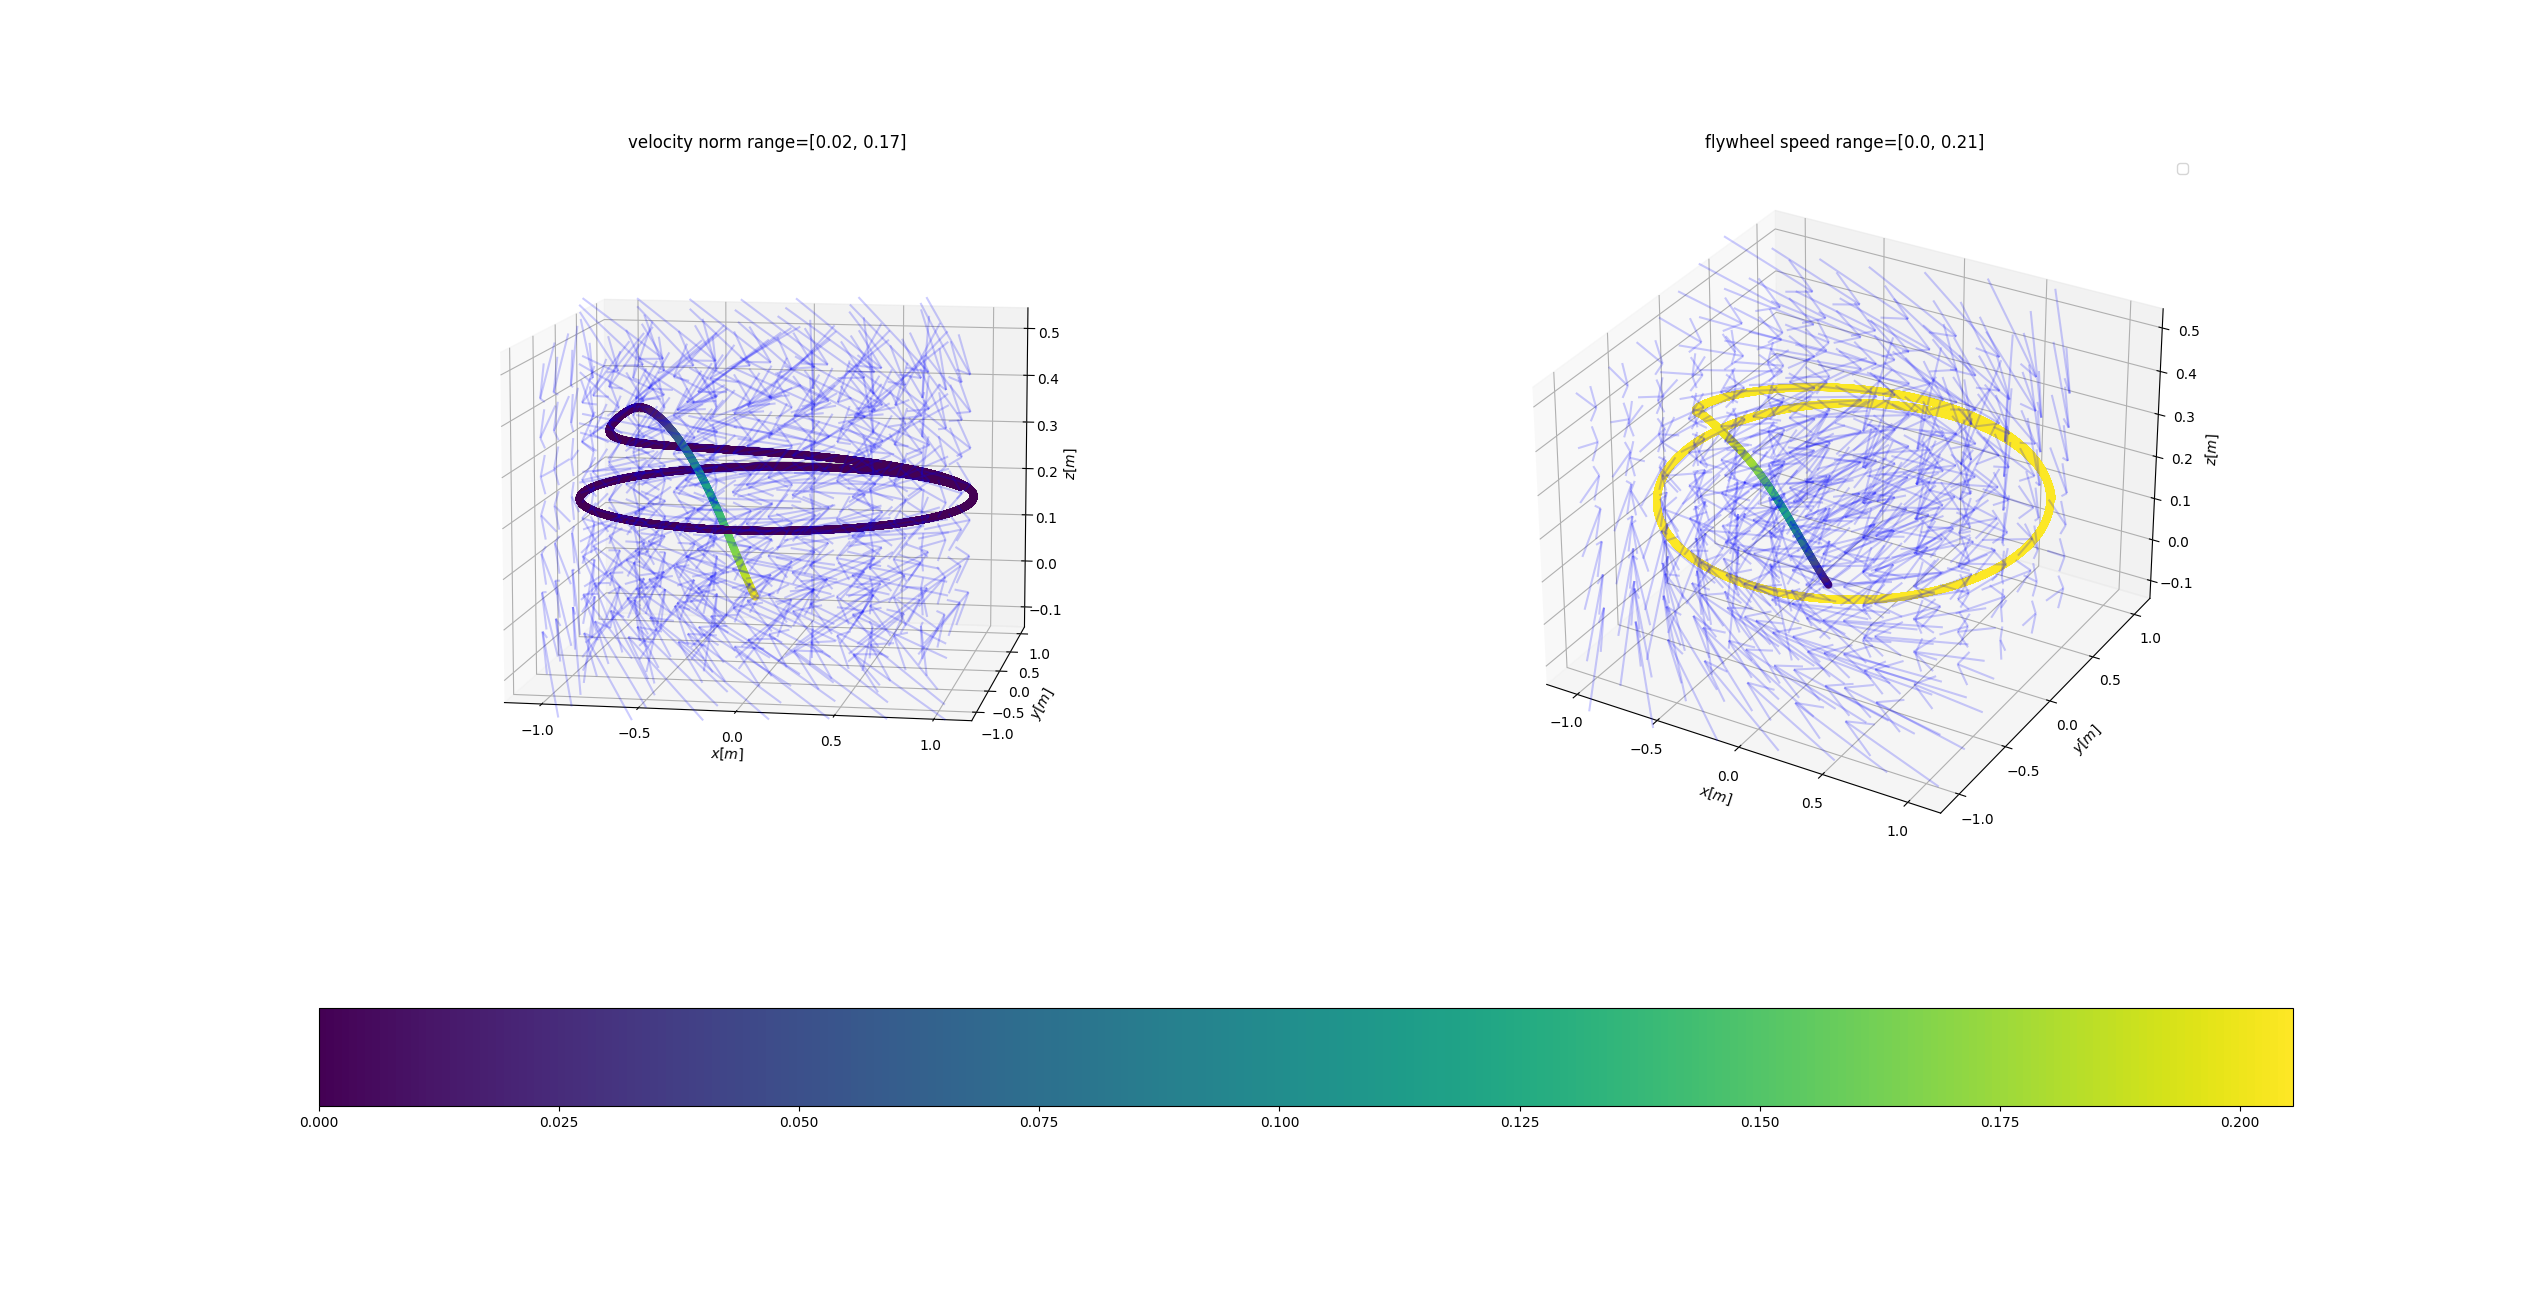
\includegraphics[width=\linewidth]{Images/python-forcecomp.png}
   \caption{trajectory and mechanical energy with force compensation }
   \label{fig:pythoncomp}
\end{figure*}
We can see in figure \ref{fig:pythoncomp} that introducing this force compensation allows the quad to continue moving despite drag forces. 
However, using such compensation slightly decreases the precision of the velocity field tracking (figure \ref{fig:trajtrackcomp}). It is not clear why this is happening.
\begin{figure}[h!]
   \centering
   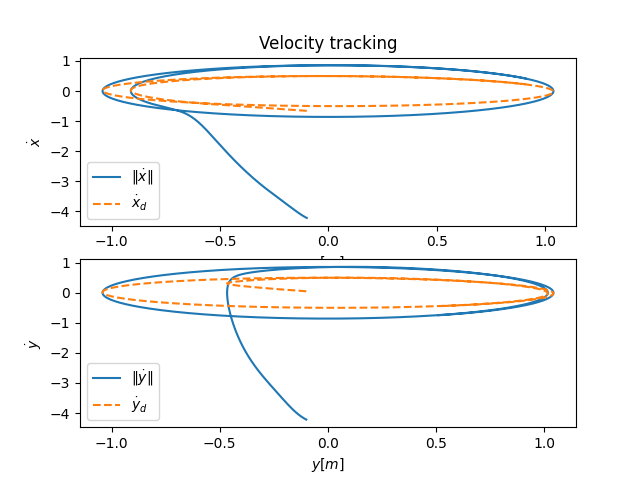
\includegraphics[width=\linewidth]{Images/velocitytrackingpythoncomp.png}
   \caption{Trajectory tracking with force compensation }
   \label{fig:trajtrackcomp}
\end{figure}

\subsection{No drag forces}
In this second experiment, we remove the drag forces from the dynamics (we set the drag coefficients to 0).
We can see in the figure \ref{fig:pythonnodrag} that when far away from the desired path, the translational speed of the quadcopter is high while the rotation speed of the flywheel is low.
This is happening because of the way the velocity field is constructed in equation \ref{eqn:circularfieldcons}, 
the magnitude of the tangential component is constant but the magnitude of the normal component is proportional to the distance between the quad and the closest point in the circle.
We can observe how energy is being traded between the quad and the flywheel when the quad approaches the desired path.
\begin{figure*}[h!]
   \centering
   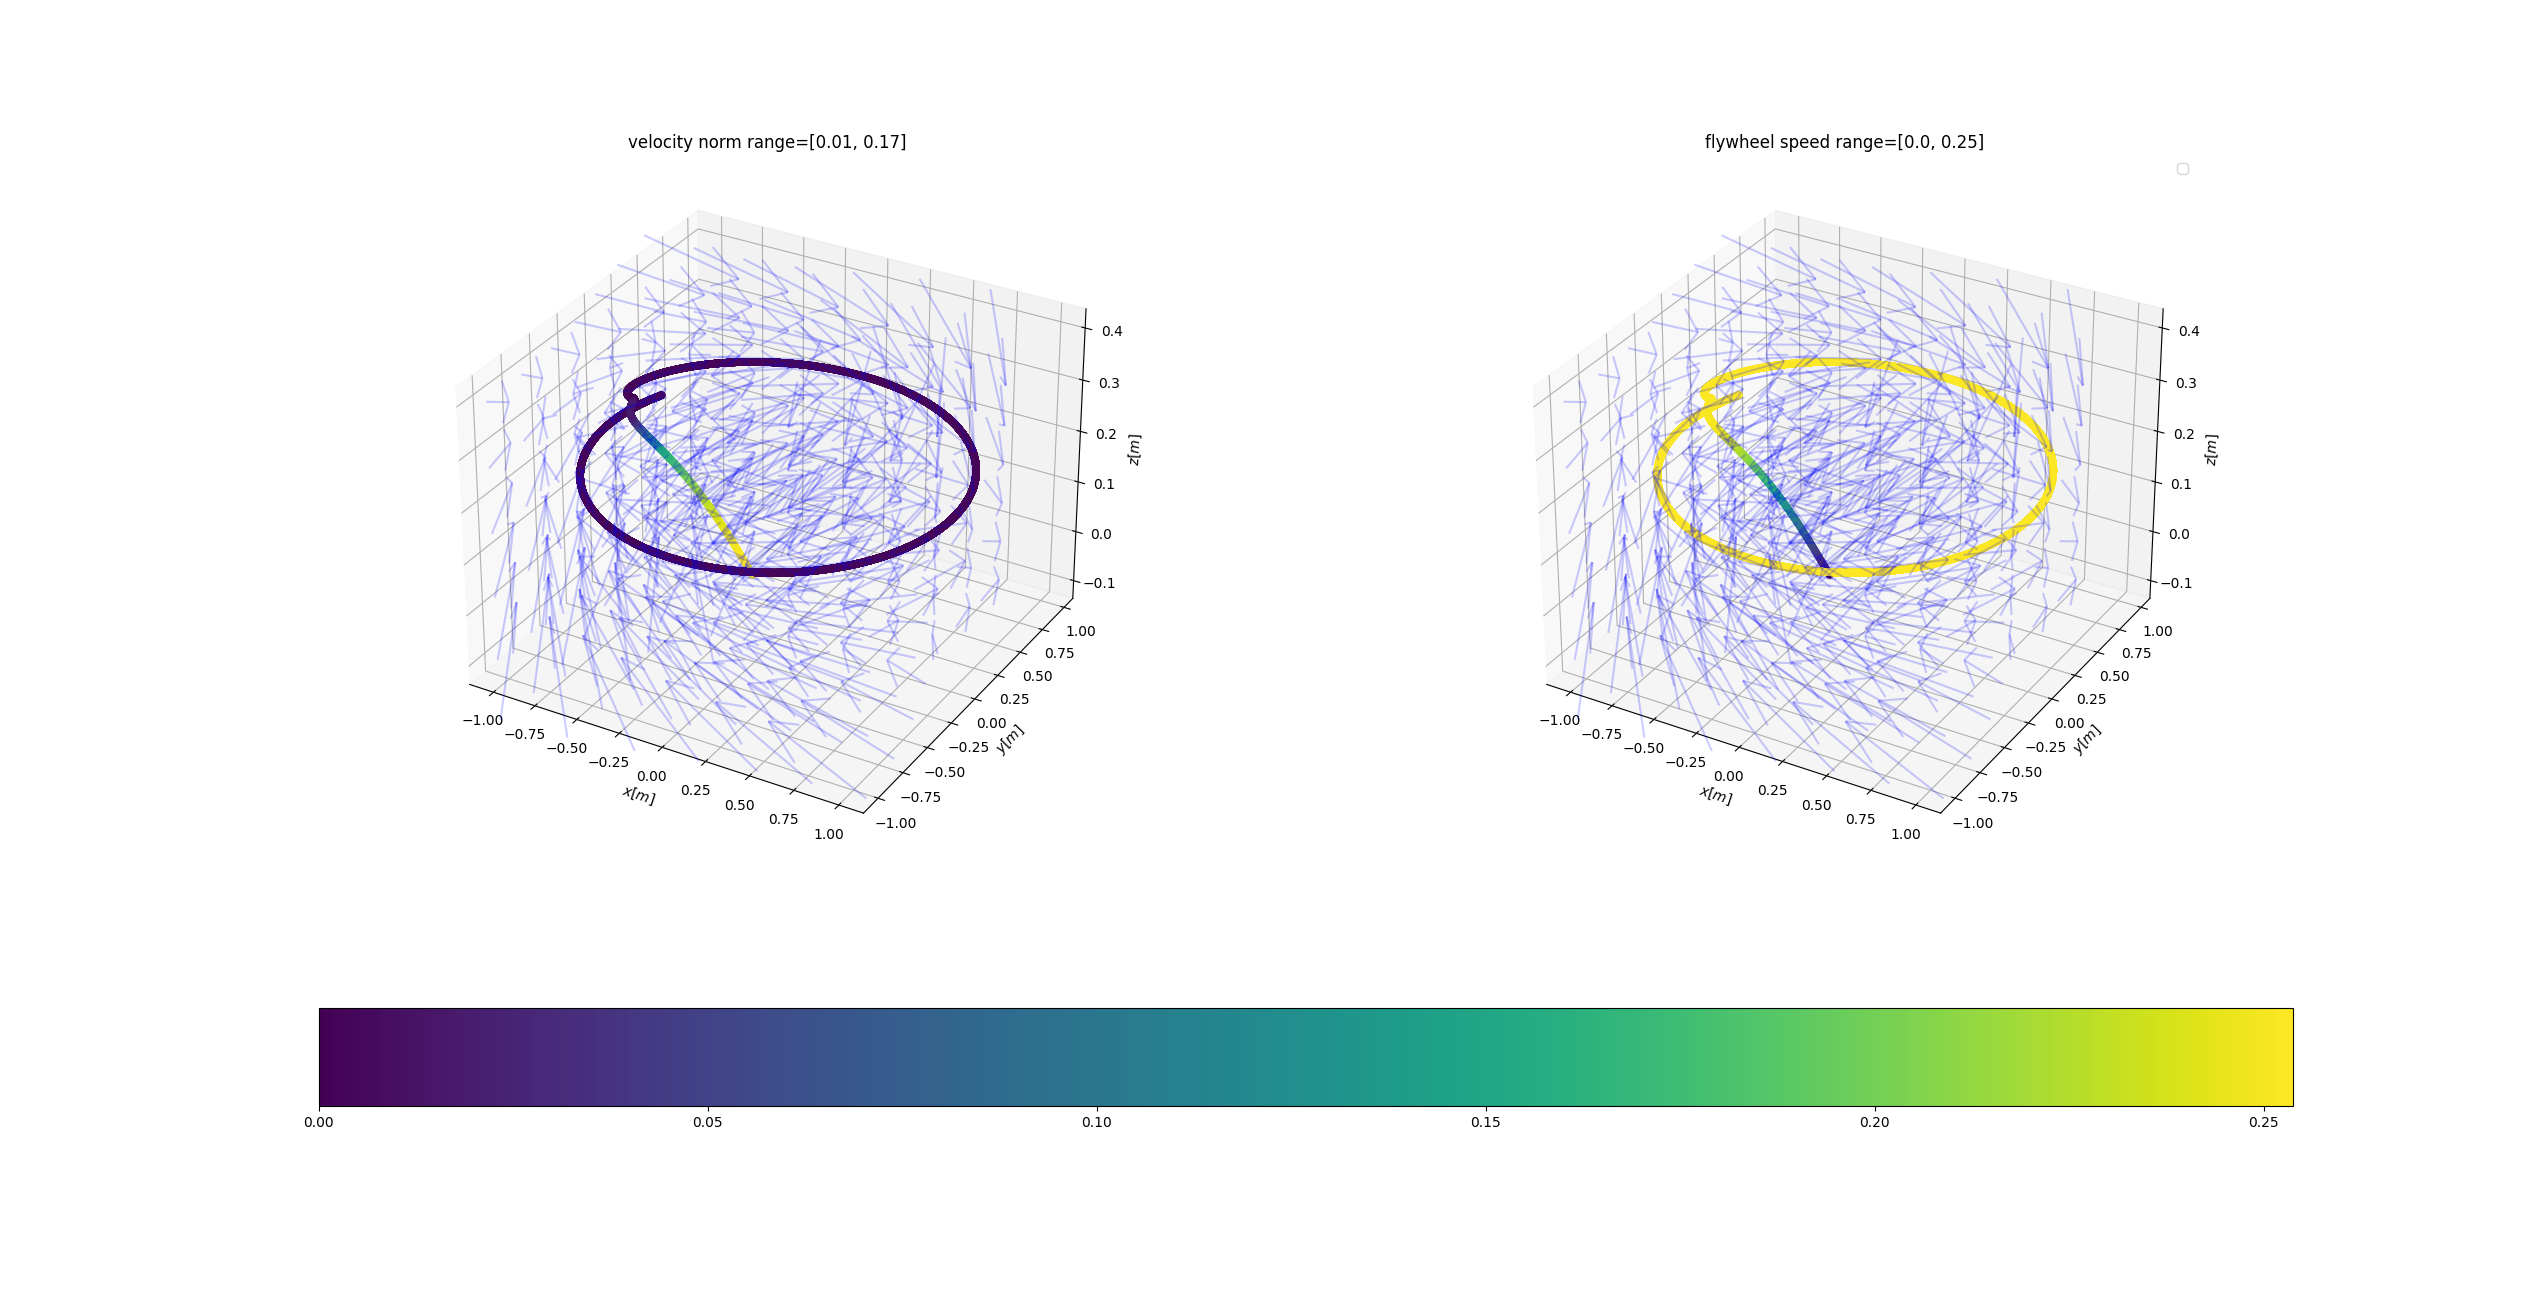
\includegraphics[width=\linewidth]{Images/python-nodrag.png}
   \caption{trajectory and mechanical energy without drag }
   \label{fig:pythonnodrag}
\end{figure*}
It should also be noted that the desired path is exactly followed in opposition to the last experiment with drag compensation (see figure \ref{fig:trajtracknodrag}).
\begin{figure}[h!]
   \centering
   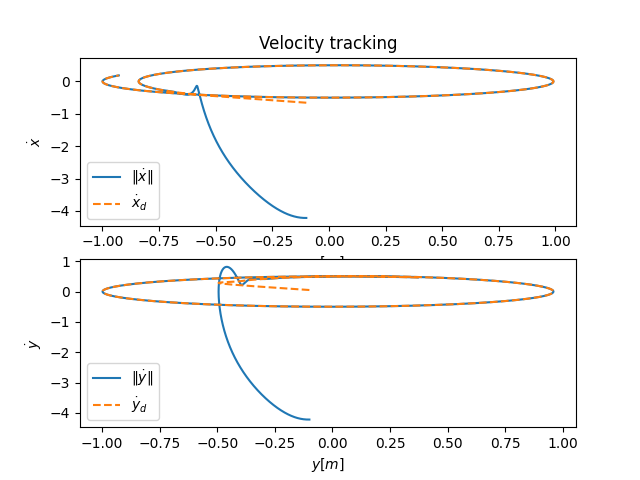
\includegraphics[width=\linewidth]{Images/velocitytrackingpythonnodrag.png}
   \caption{Trajectory tracking without drag}
   \label{fig:trajtracknodrag}
\end{figure}
We explained in section 3 that PVFC has interesting properties regarding the velocity tracking error (eq \ref{alphaerror}). 
In \cite{li1999passive}, the author explains that when no external forces are applied on the quadcopter, $\alpha$ should approach the square root of $\beta^2 = \frac{\text{augmented mechanical energy}}{\text{augmented desired mechanical energy}}$.\\
In addition, when $\alpha$ approaches $\beta$, the $\alpha$ error should approach 0.

\begin{figure}[h!]
   \centering
   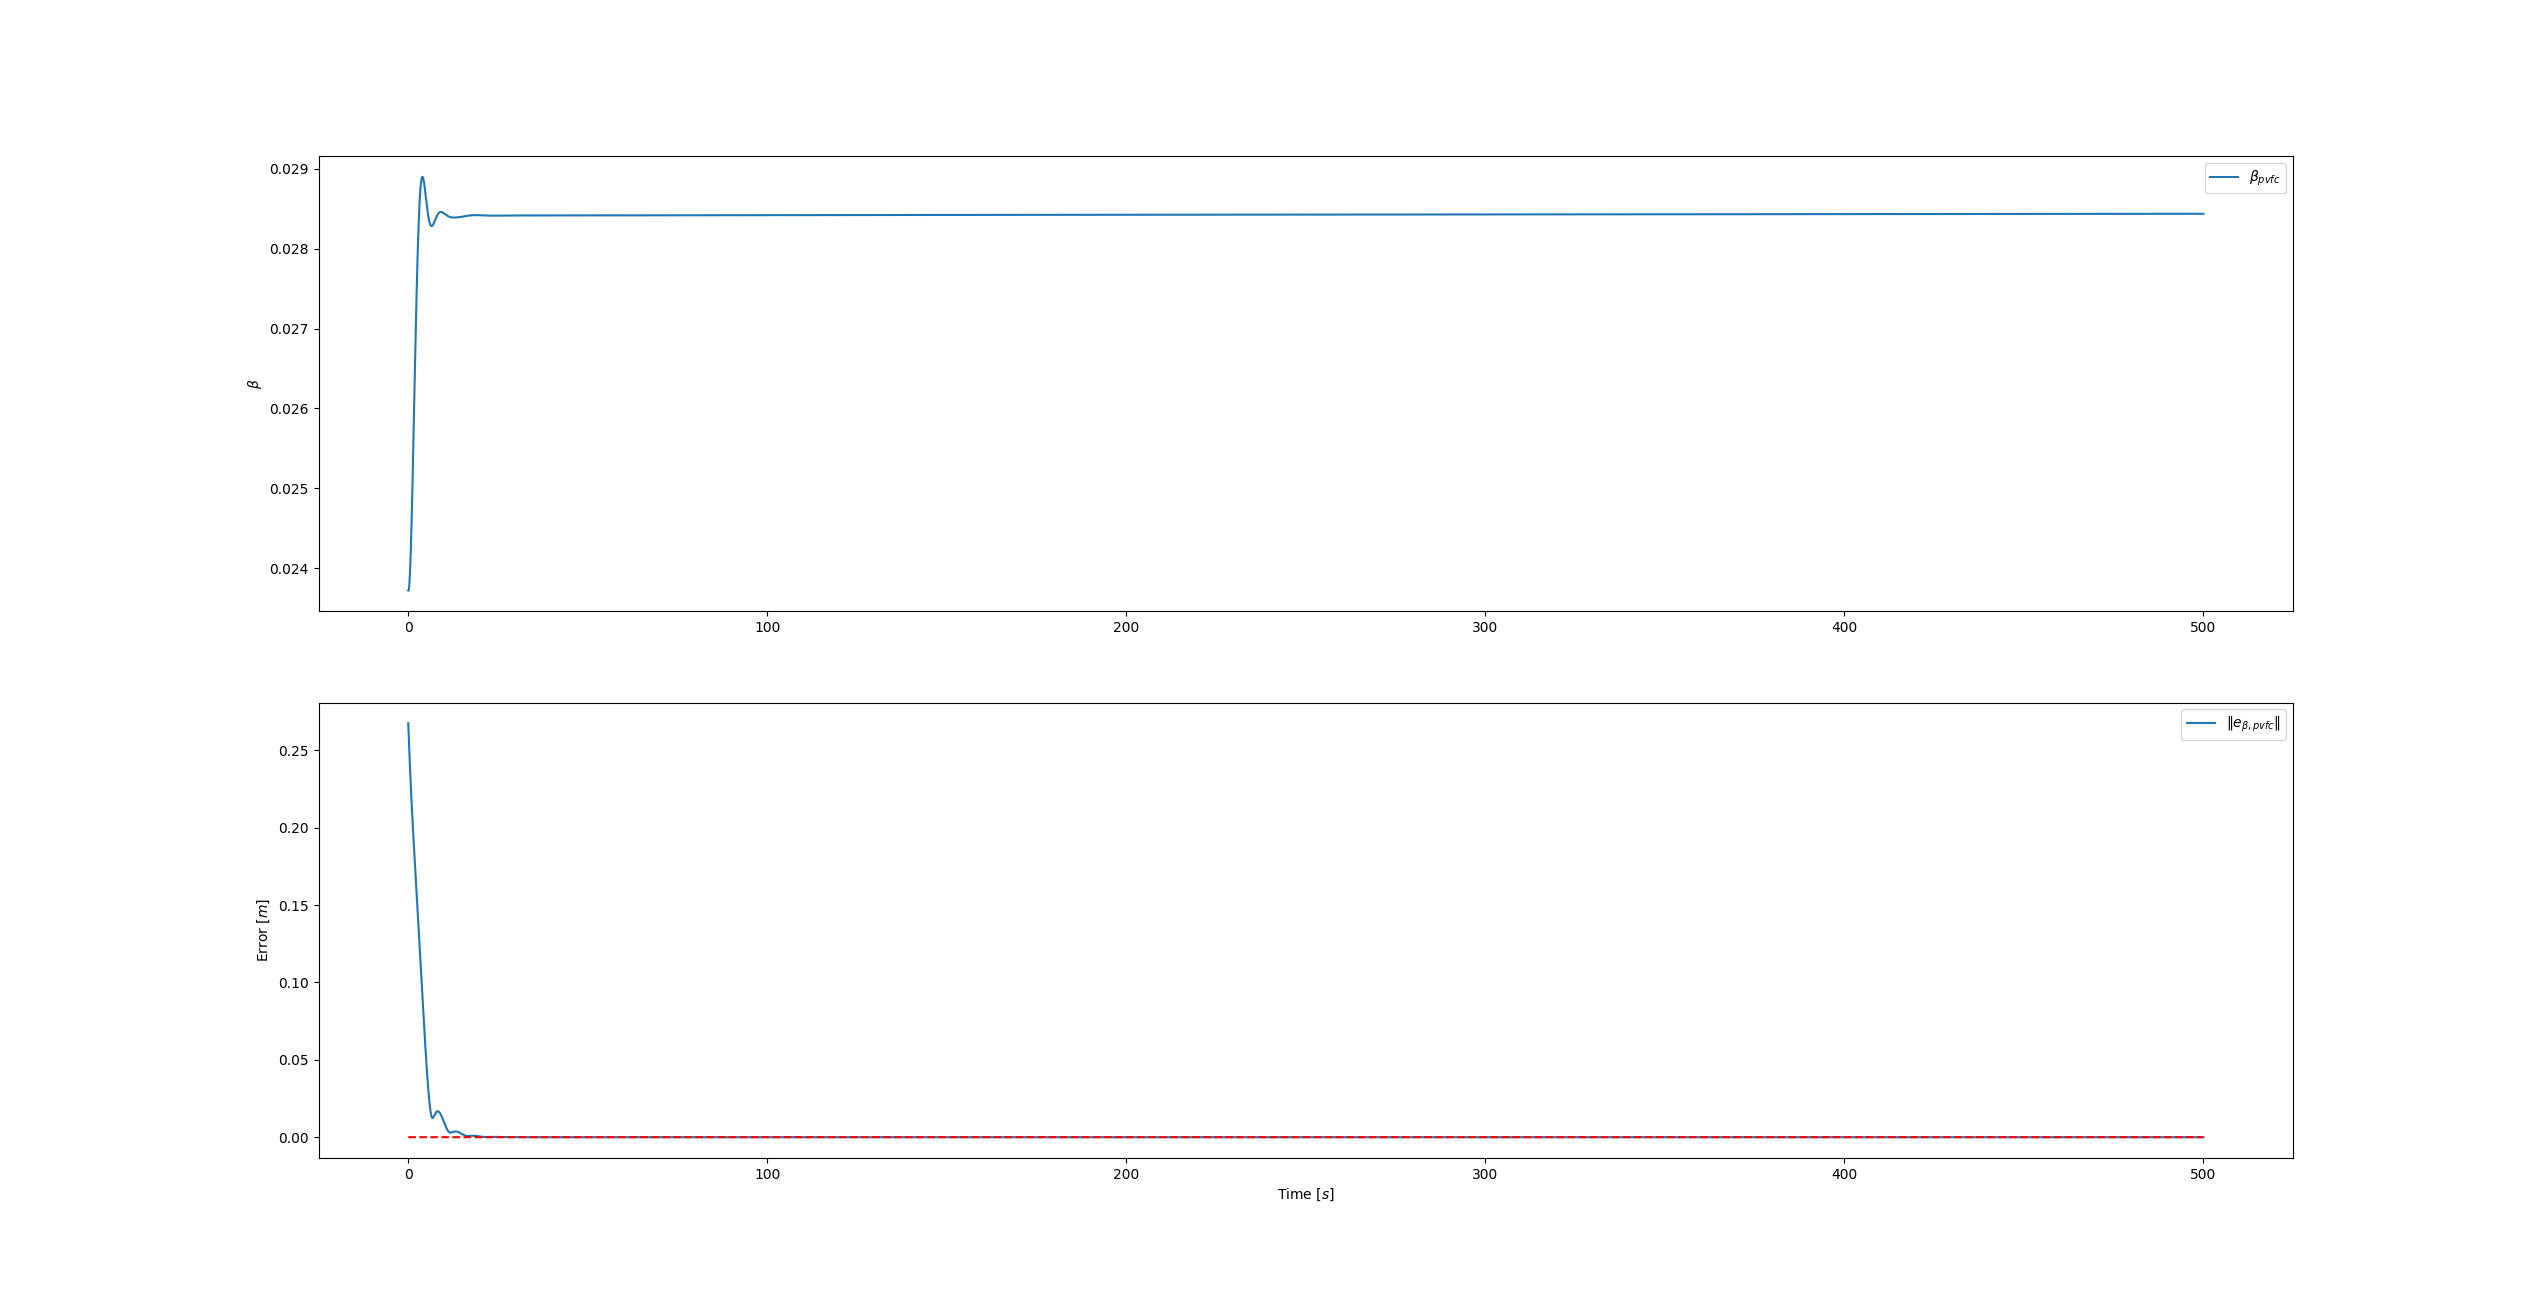
\includegraphics[width=\linewidth, scale=1.5]{Images/betaerrornodrag.png}
   \caption{Beta error without drag}
   \label{fig:betaerrornodrag}
\end{figure}
By design, the augmented desired mechanical energy of the system is always equal to $\bar{E}$, and we compute the augmented mechanical energy given by:\\
$\frac{1}{2}m_b\lVert\dot{q}\rVert^2 + \frac{1}{2}m_{fly}\lVert\dot{q}_{fly}\rVert^2 $. \\
We successfully reproduced the results of \cite{li1999passive} for the $\beta$ error on a circular velocity field. We can see in figure \ref{fig:betaerrornodrag} that $\beta$ converges and the $\beta$ error converges to 0.

\subsection{No drag forces with force wrench}
The third experiment is done in 3 phases: In the first one we let the quad follow the circular field for 120 seconds, 
then we apply an external force on the quad in the $-\hat{y}$ direction for 10 seconds,
and finally we let the quad follow the desired field for 120 seconds.
\begin{figure*}[h!]
   \centering
   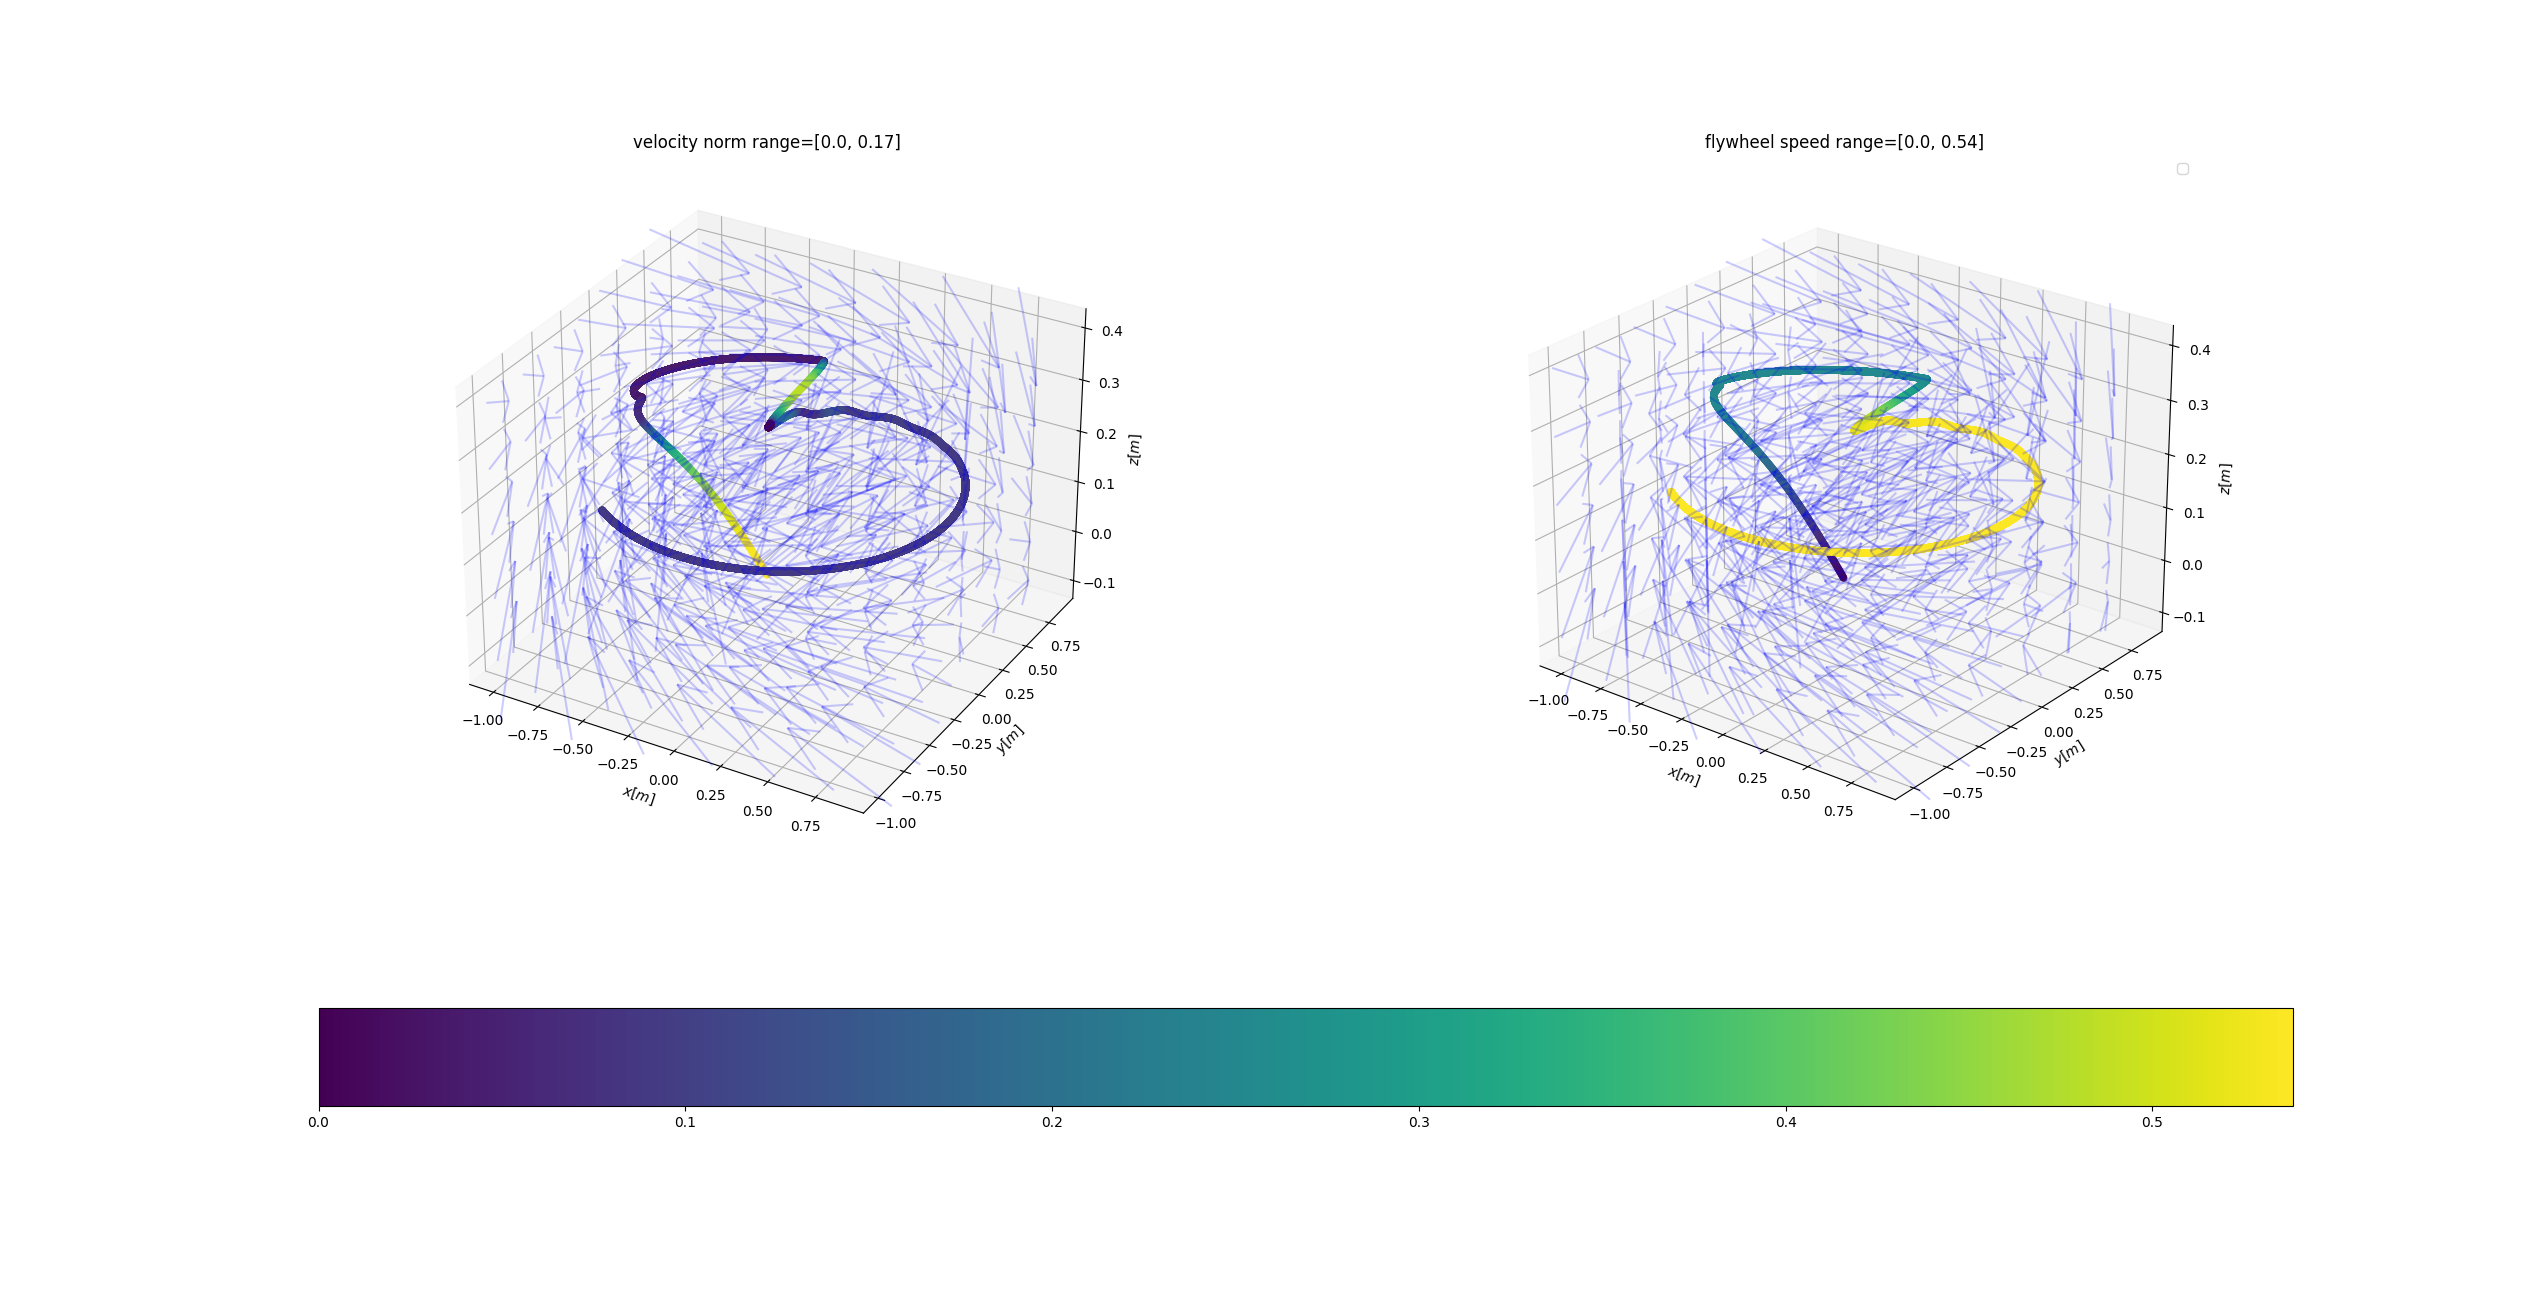
\includegraphics[width=\linewidth]{Images/python-nodrag-wrench.png}
   \caption{trajectory and mechanical energy without drag and with wrench - Python POC }
   \label{fig:pythonnodragwrench}
\end{figure*}
The passivity properties of PVFC are well shown in figure \ref{fig:pythonnodragwrench}. We can see how the quadcopter is trading energy with the environement and dissipating the work of the wrench inside the augmented system.
This experiment also exemplifies well the advantage of using velocity field instead of a traditional trajectory following based controller:
\begin{figure}[h!]
   \centering
   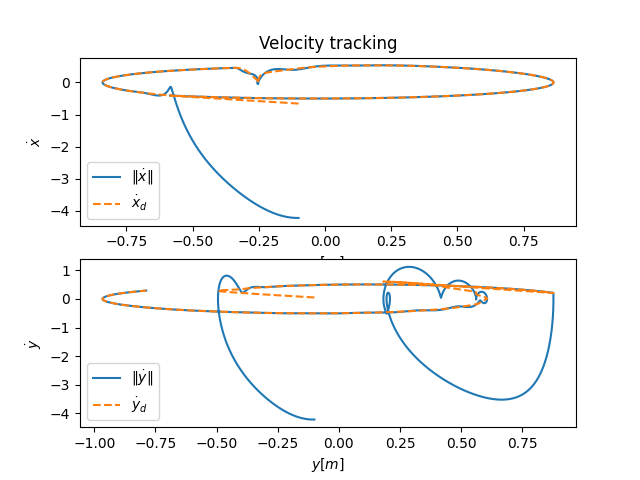
\includegraphics[width=\linewidth]{Images/velocitytrackingpythonnodragwrench.png}
   \caption{Trajectory tracking without drag with wrench - Python POC }
   \label{fig:trajtracknodragwrench}
\end{figure}
The radial reduction that could have occured in figure \ref{fig:trajtracknodragwrench} could have been a big issue in a task such as contour following where following the contour is more important than following a trajectory.
In the contrary, figure \ref{fig:trajtracknodragwrench} shows that when external forces are applied, we are able to go back to the desired circular path without radial reduction.
In addition, we can observe what happens to the $\beta$ error when wrench is applied:
\begin{figure}[h!]
   \centering
   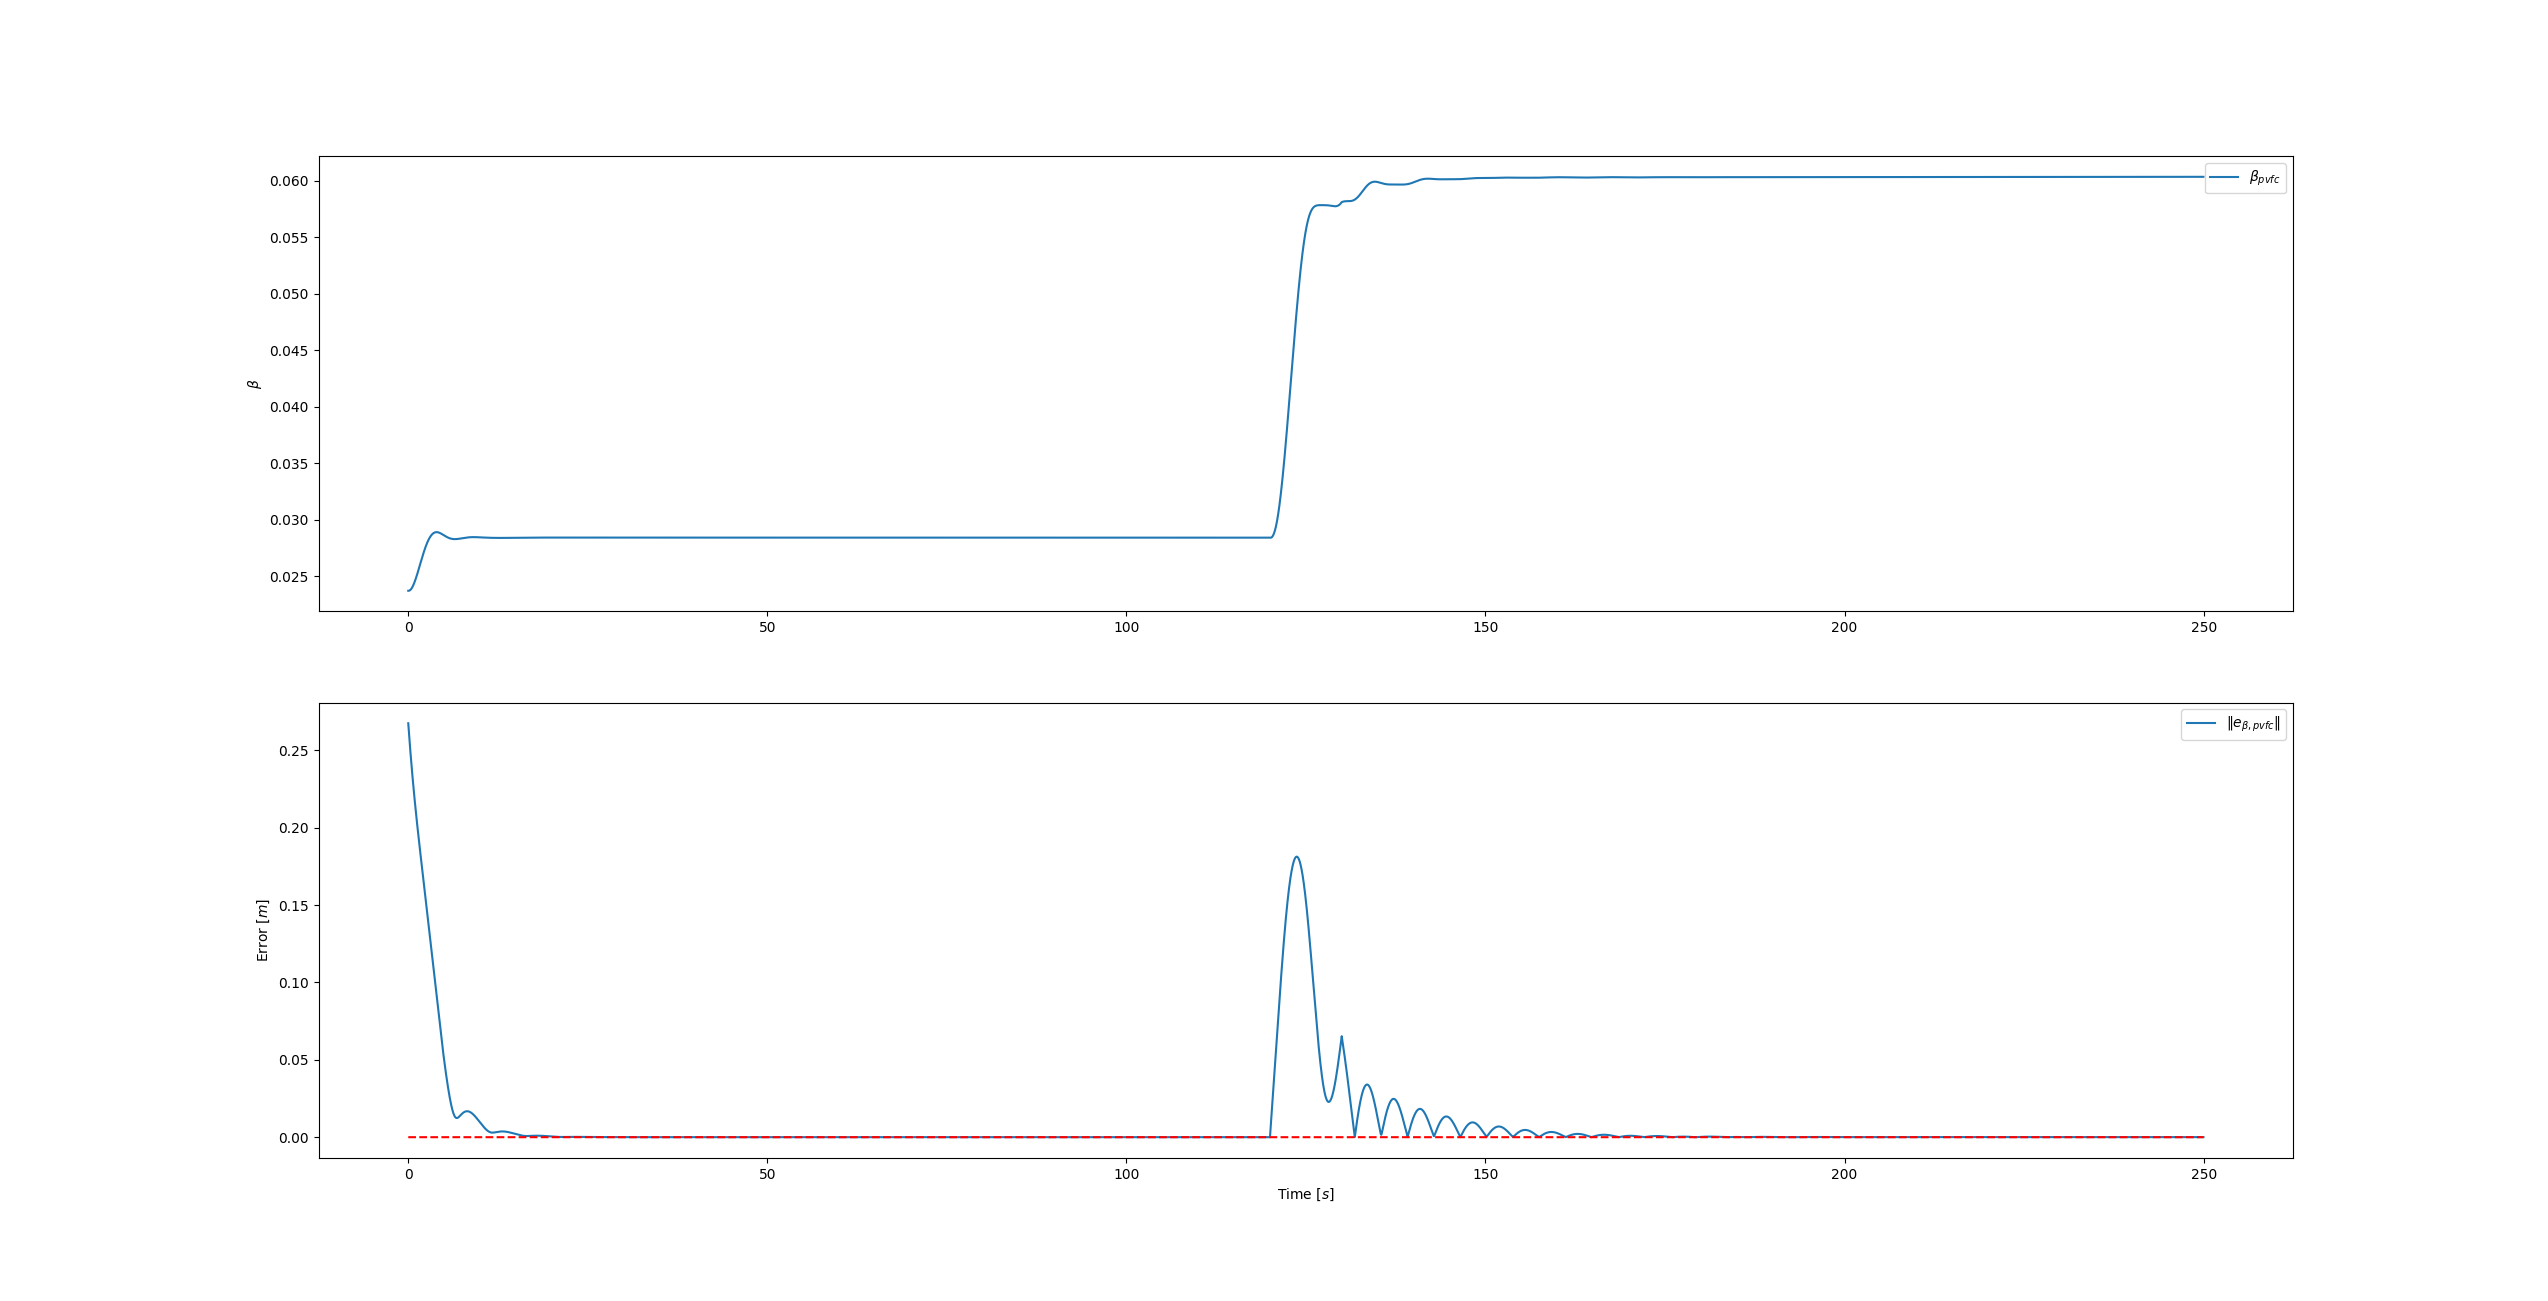
\includegraphics[width=\linewidth, scale=1.5]{Images/betaerrornodragwrench.png}
   \caption{Beta error without drag with wrench}
   \label{fig:betaerrornodragwrench}
\end{figure}
We can see in figure \ref{fig:betaerrornodragwrench} that the $\beta$ error converges to 0 before a wrench is applied, 
then during the second phase, we can see a spike for both $\beta$ and $\beta$ error when a wrench is applied. This is expected since the wrench increases mechanical energy in the system. 
We can see how PVFC dissipates the external force and makes the $\beta$ error converge to 0 when no external force is applied in the last phase.

Now we are going to show experiments done on the Gazebo simulation.
In the scatter trajectory plot that we will see in the following experiment, the color represents the velocity of the flywheel.
\subsection{Circular Field}
This subsection contains graphs and experiment with the circular field planner.
\subsubsection{$\bar{E}$ study}
In this subsubsection, we try to gain intuition about the $\bar{E}$ parameter of the controller with the circular velocity field.
Let us remember that $\bar{E}$ is the (desired) energy reservoir of the system such that the desired total mechanical of the system (meaning, the desired kinetic energy in the flywheel plus the desired kinetic energy coming from the desired translational velocity of the quadcopter).
$\bar{E}$ is used in 2 places: The first is in the velocity field code where the flywheel velocity field is computed according to equation \ref{eqn:vfly}, the second one when computing $\tau_c$ in the coupling control law \ref{tauc}.
We can see in figures \ref{fig:trajgazebocircularebar} and \ref{fig:velgazebocircularebar} that the velocity of the quadcopter with the lowest $\bar{E}$ is the highest.
This is expected since the amplitude of $\tau_c$ is inverse proportional to $\bar{E}$
\begin{figure*}[h!]
   \centering
   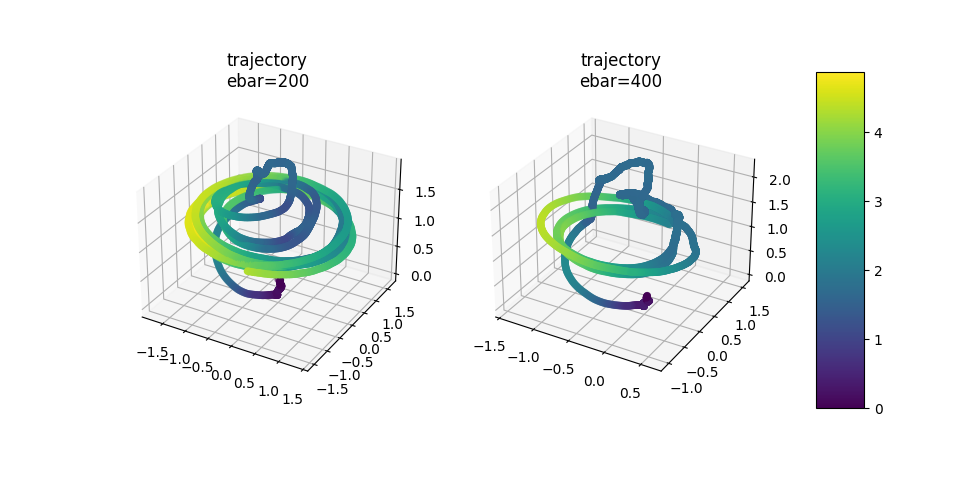
\includegraphics[width=\linewidth]{Images/gazebo_trajectory_ebar_circular.png}
   \caption{circular field trajectory Gazebo - $\bar{E}$ experiment}
   \label{fig:trajgazebocircularebar}
\end{figure*}
\begin{figure*}[h!]
   \centering
   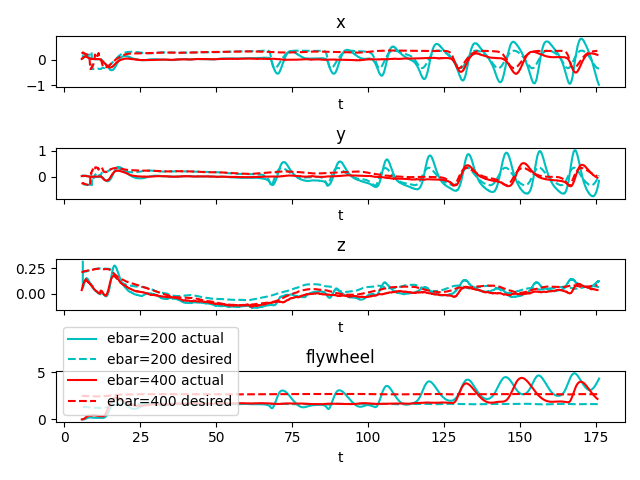
\includegraphics[width=\linewidth]{Images/gazebo_circular_ebar_V.png}
   \caption{circular field velocity comparison Gazebo - $\bar{E}$ experiment}
   \label{fig:velgazebocircularebar}
\end{figure*}
\subsubsection{$\gamma$ study}
The $\gamma$ parameter of PVFC controls the amplide of the feedback term of the PVFC control law \ref{tauf}.
We would expect to follow the desired velocity field more accuratly when $\gamma$ is higher.
As we can see in figure \ref{fig:trajgazebocirculargamma}, the circles are draw more accurately for $\gamma=0.5$.
When the field is not smooth enough, increasing gamma may cause instability because the desired attitude will change faster according to the direction of the desired
velocity field and if those changes are too fast, the quad may turn over on its back and fall to the ground. The root cause of this problem is that $\gamma$ can be seen as a proportional gain (\ref{eqn:pid}) and setting it too high without a derivative and integral term causes instability in the control loop and the quad attitude.
We can also from figure \ref{fig:betaerrorgazebocirculargamma} that the higher the $\gamma$ the lower the $\beta$ error. This is expected as higher $\gamma$ (to some extent, after some threshold the system becauses instable) means faster convergence to the desired velocity field.

\begin{figure*}[h!]
   \centering
   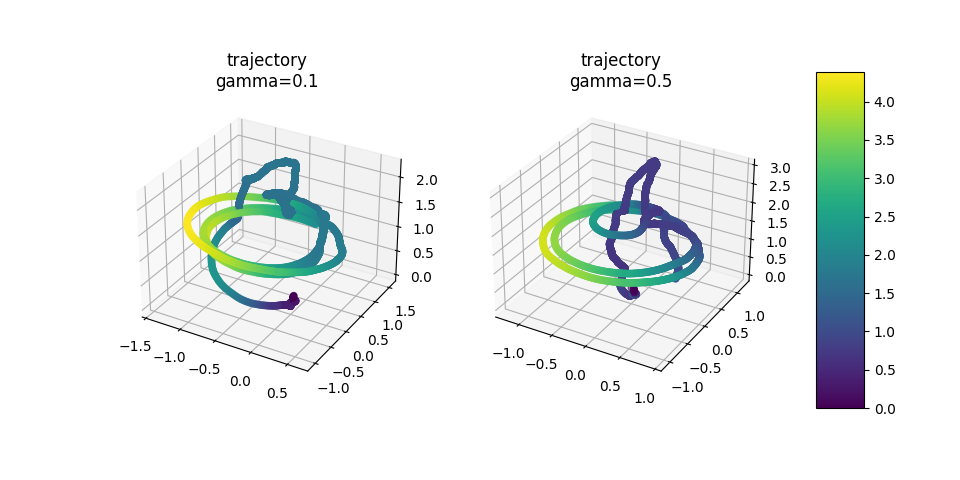
\includegraphics[width=\linewidth]{Images/gazebo_trajectory_gamma_circular.png}
   \caption{circular field trajectory Gazebo - $\gamma$ experiment}
   \label{fig:trajgazebocirculargamma}
\end{figure*}
\begin{figure*}[h!]
   \centering
   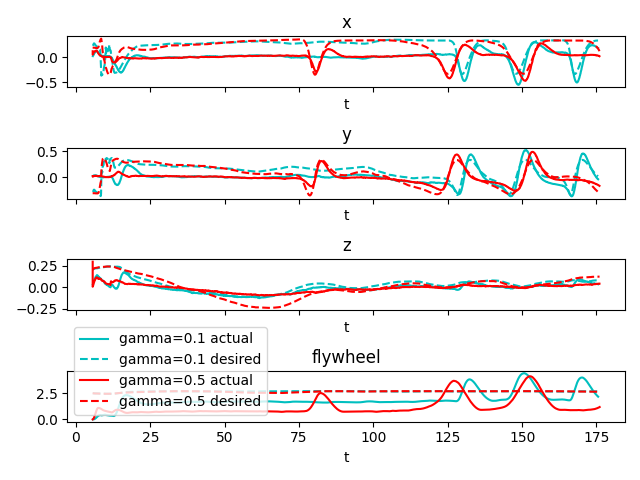
\includegraphics[width=\linewidth]{Images/gazebo_circular_gamma_V.png}
   \caption{circular field velocity comparison Gazebo - $\gamma$ experiment}
   \label{fig:velgazebocirculargamma}
\end{figure*}
\begin{figure*}[h!]
   \centering
   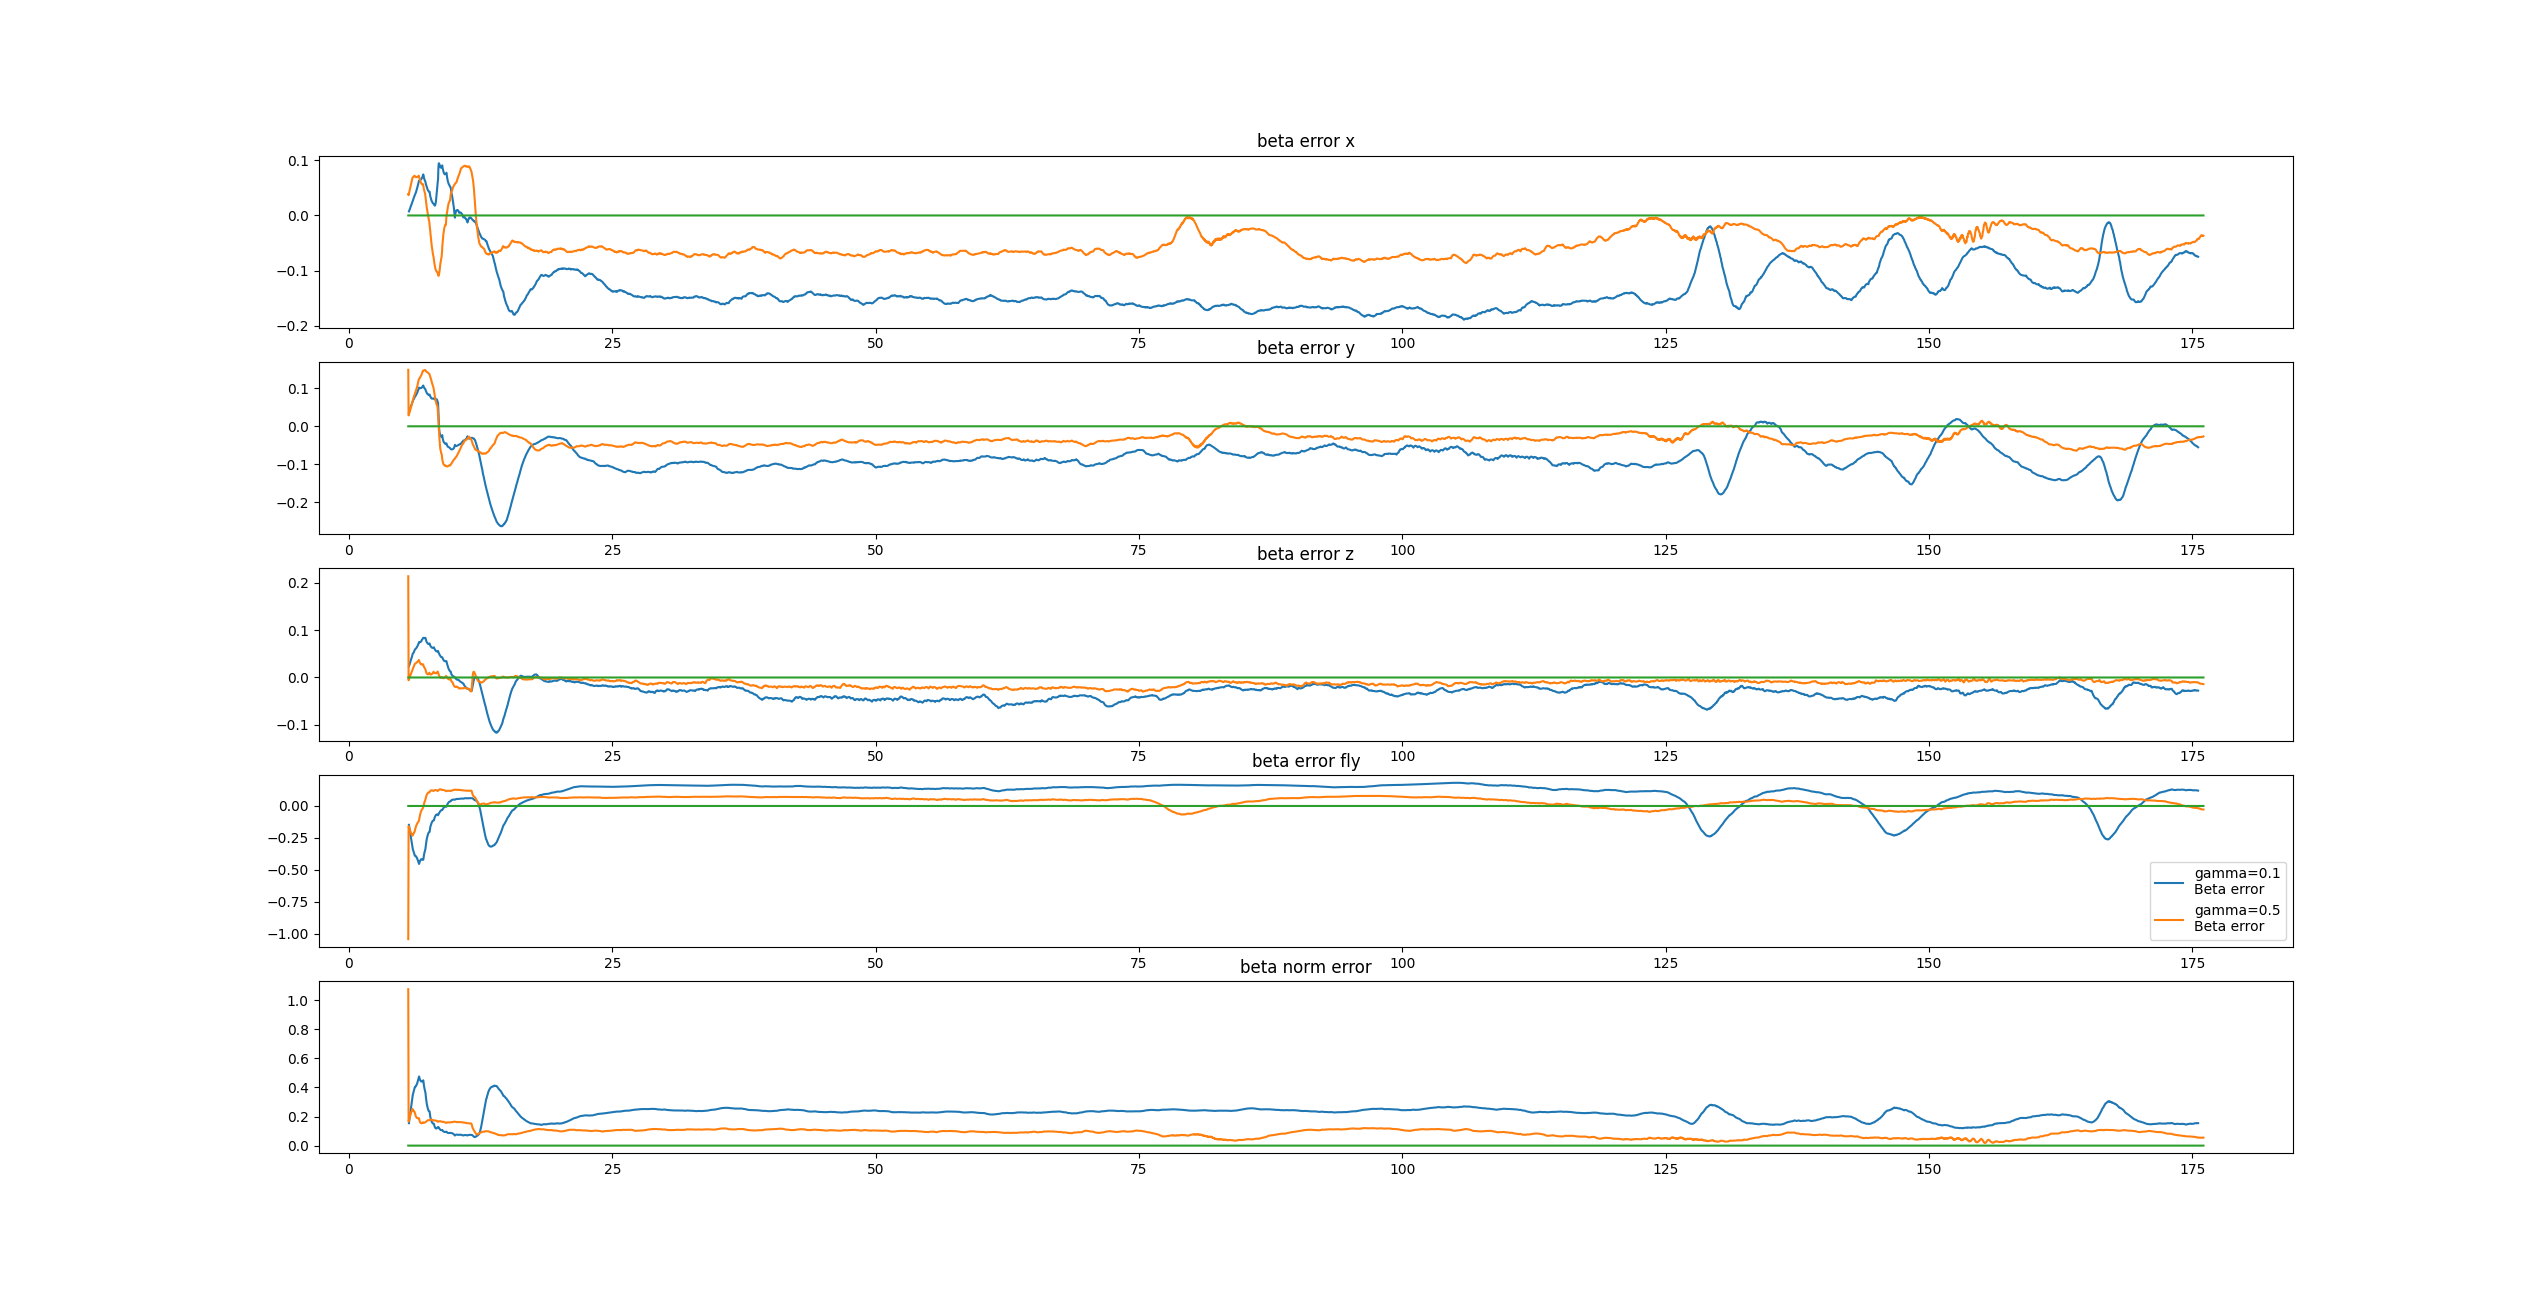
\includegraphics[width=\linewidth]{Images/gazebo_betaerror_gamma_circular.png}
   \caption{circular field $\beta$ error Gazebo - $\gamma$ experiment}
   \label{fig:betaerrorgazebocirculargamma}
\end{figure*}
\subsubsection{force compensation study}
As we previously explained, the force compensation is essential when drag forces are in presence. 
It is important to remember that in the Python implementation, the dynamics of the drag forces are linear with respect to the speed of the quadcopter but in Gazebo, 
the drag forces are more complex and not linear to the velocity of the moving body. Therefore, it is hard to find the right linear drag coefficient that will approximate the Gazebo drag force on the IRIS model.
We can see how essential is this compensation term in the figures \ref{fig:velgazebocircularfcomp} and \ref{fig:trajgazebocircularfcomp}, without drag force compensation, the trajectory is not circular at all and the mechanical energy in the system goes to 0. 
\begin{figure*}[h!]
   \centering
   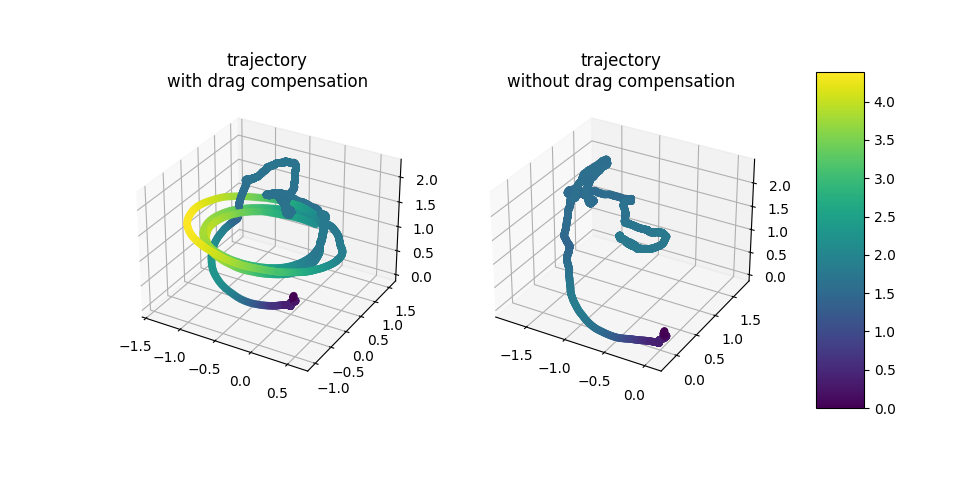
\includegraphics[width=\linewidth]{Images/gazebo_trajectory_fcomp_circular.png}
   \caption{circular field trajectory Gazebo - drag compensation experiment}
   \label{fig:trajgazebocircularfcomp}
\end{figure*}
\begin{figure*}[h!]
   \centering
   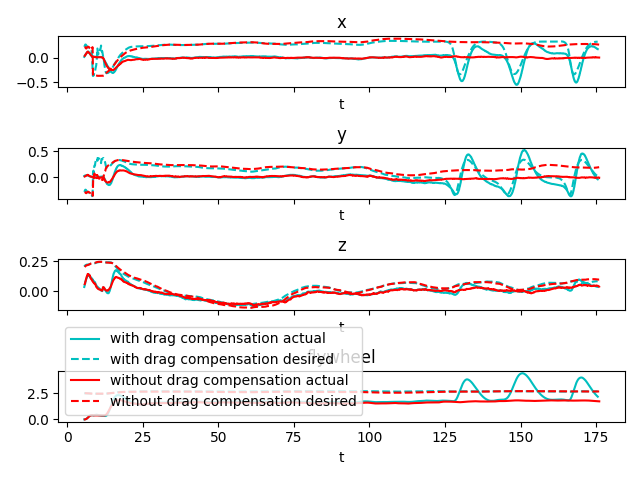
\includegraphics[width=\linewidth]{Images/gazebo_circular_fcomp_V.png}
   \caption{circular field velocity comparison Gazebo - drag compensation experiment}
   \label{fig:velgazebocircularfcomp}
\end{figure*}
\subsubsection{World with Wrench}
In the above Gazebo experiments, no external force (except drag) was applied on the system. 
We present here an experiment where a force wrench was applied on the quadcopter during 5 seconds. 
We will compare it with an experiment in the same conditions but without force wrench applied.
\begin{figure*}[h!]
   \centering
   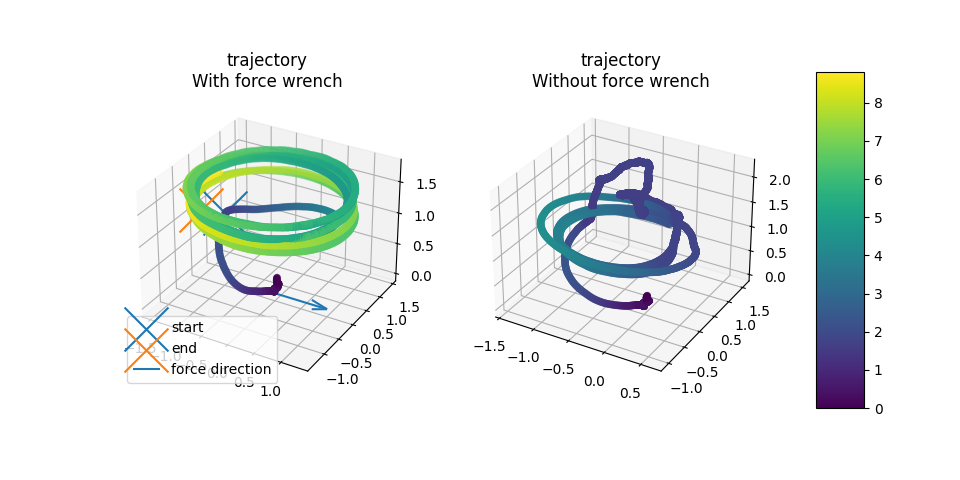
\includegraphics[width=\linewidth]{Images/gazebo_trajectory_wrench_circular.png}
   \caption{circular field trajectory Gazebo - Wrench experiment}
   \label{fig:trajgazebocircularfwrench}
\end{figure*}
\begin{figure*}[h!]
   \centering
   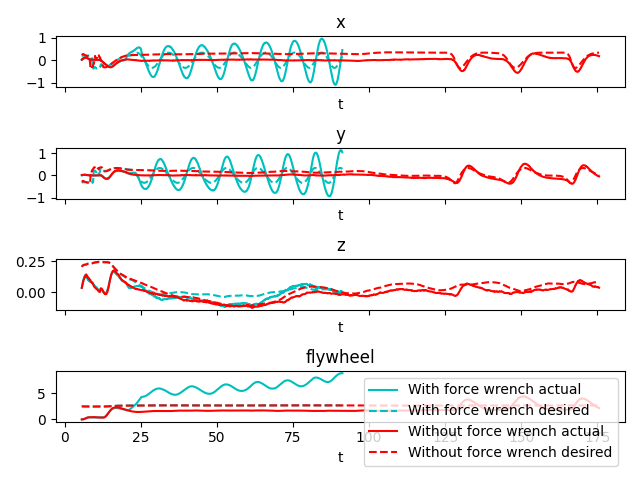
\includegraphics[width=\linewidth]{Images/gazebo_circular_wrench_V.png}
   \caption{circular field velocity comparison Gazebo - Wrench experiment}
   \label{fig:velgazebocircularfwrench}
\end{figure*}
We can see in figure \ref{fig:trajtracknodragwrench} that the wrench is injecting energy into the augmented system and that PVFC performs much better in term of velocity field tracking when it is dissipating this external work inside the augmented system. 
This experience also motivates injecting an initial energy into the system. However, it is hard to finetune the linear drag coefficient together with the amount of injected energy.
We could not run the wrench experiment for more than 100 seconds because the quad crashes. We can see one of the reasons why the crash occurs in figure \ref{fig:velgazebocircularfwrench}: The velocity of the flywheel is diverging, and the translational velocity of the quadcopter is also increasing. 
This experiments shows that it is crucial to carefully select the linear drag terms because we might lose the passivity properties of the controller when it is too high.
This experiments also shows how robust the controller is for passive contour following when external forces are applied on the quadcopter.
A \href{https://youtu.be/NcAQGyCOlOk}{video} of this experiment is available on Youtube
\subsection{Potential sink Field}
In the following experiment, we will study the behavior of PVFC when the desired velocity field is the sink potential field described in section 3.
In this section, PVFC will be under the regime of 2 successive potential sink field: The first one is a sink at point $(0,0,0.5)$ (only $+\hat{z}$) to gain altitude and
the second one is a sink at point $(5,0,0.5)$ to reach the desired target point. 
It should be noted that the linear force compensation had to be increased in the potential sink experiments to accuratly follow the desired field.
This may be caused by the decreasing norm of the potential field when approaching the desired target point while the norm of the circular field is only affected by the distance from the quad to the closest point on the circle.  
\subsubsection{$\bar{E}$ study}
\begin{figure}[h!]
   \centering
   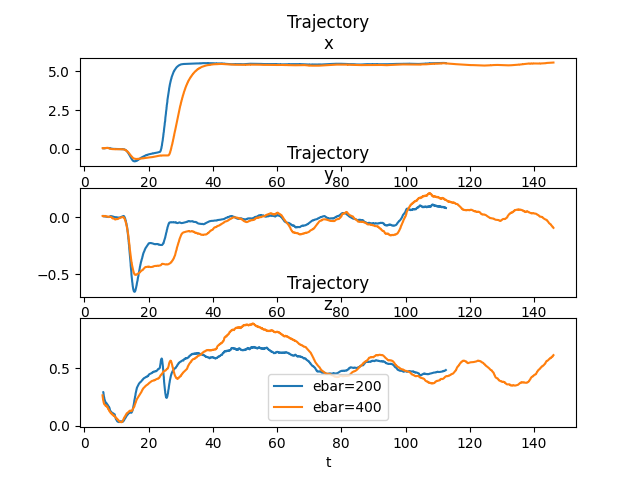
\includegraphics[width=\linewidth]{Images/gazebo_trajectory_ebar_potential_2d.png}
   \caption{potential field velocity 2d trajectory comparison Gazebo - ebar experiment}
   \label{fig:vel2dgazeboebarpotential}
\end{figure}
We can see that the trajectory in the $\hat{x}$ and $\hat{y}$ axis are more stable around the desired state when $\bar{E}=200$.
However, if we set $\bar{E}$ to be too small, the desired speed of the flywheel (\ref{eqn:vfly}) may not be a real number which will cause the controller to stop working.
Therefore, it is important to finetune this parameter according to the desired velocity field such that it would be the minimum necessary to have a real flywheel desired velocity.
It should also be noted that the spike in the $\beta$ error when switching field is higher when $\bar{E}$ is small (see figure \ref{fig:betaerrorgazebopotentialebar})
\begin{figure*}[h!]
   \centering
   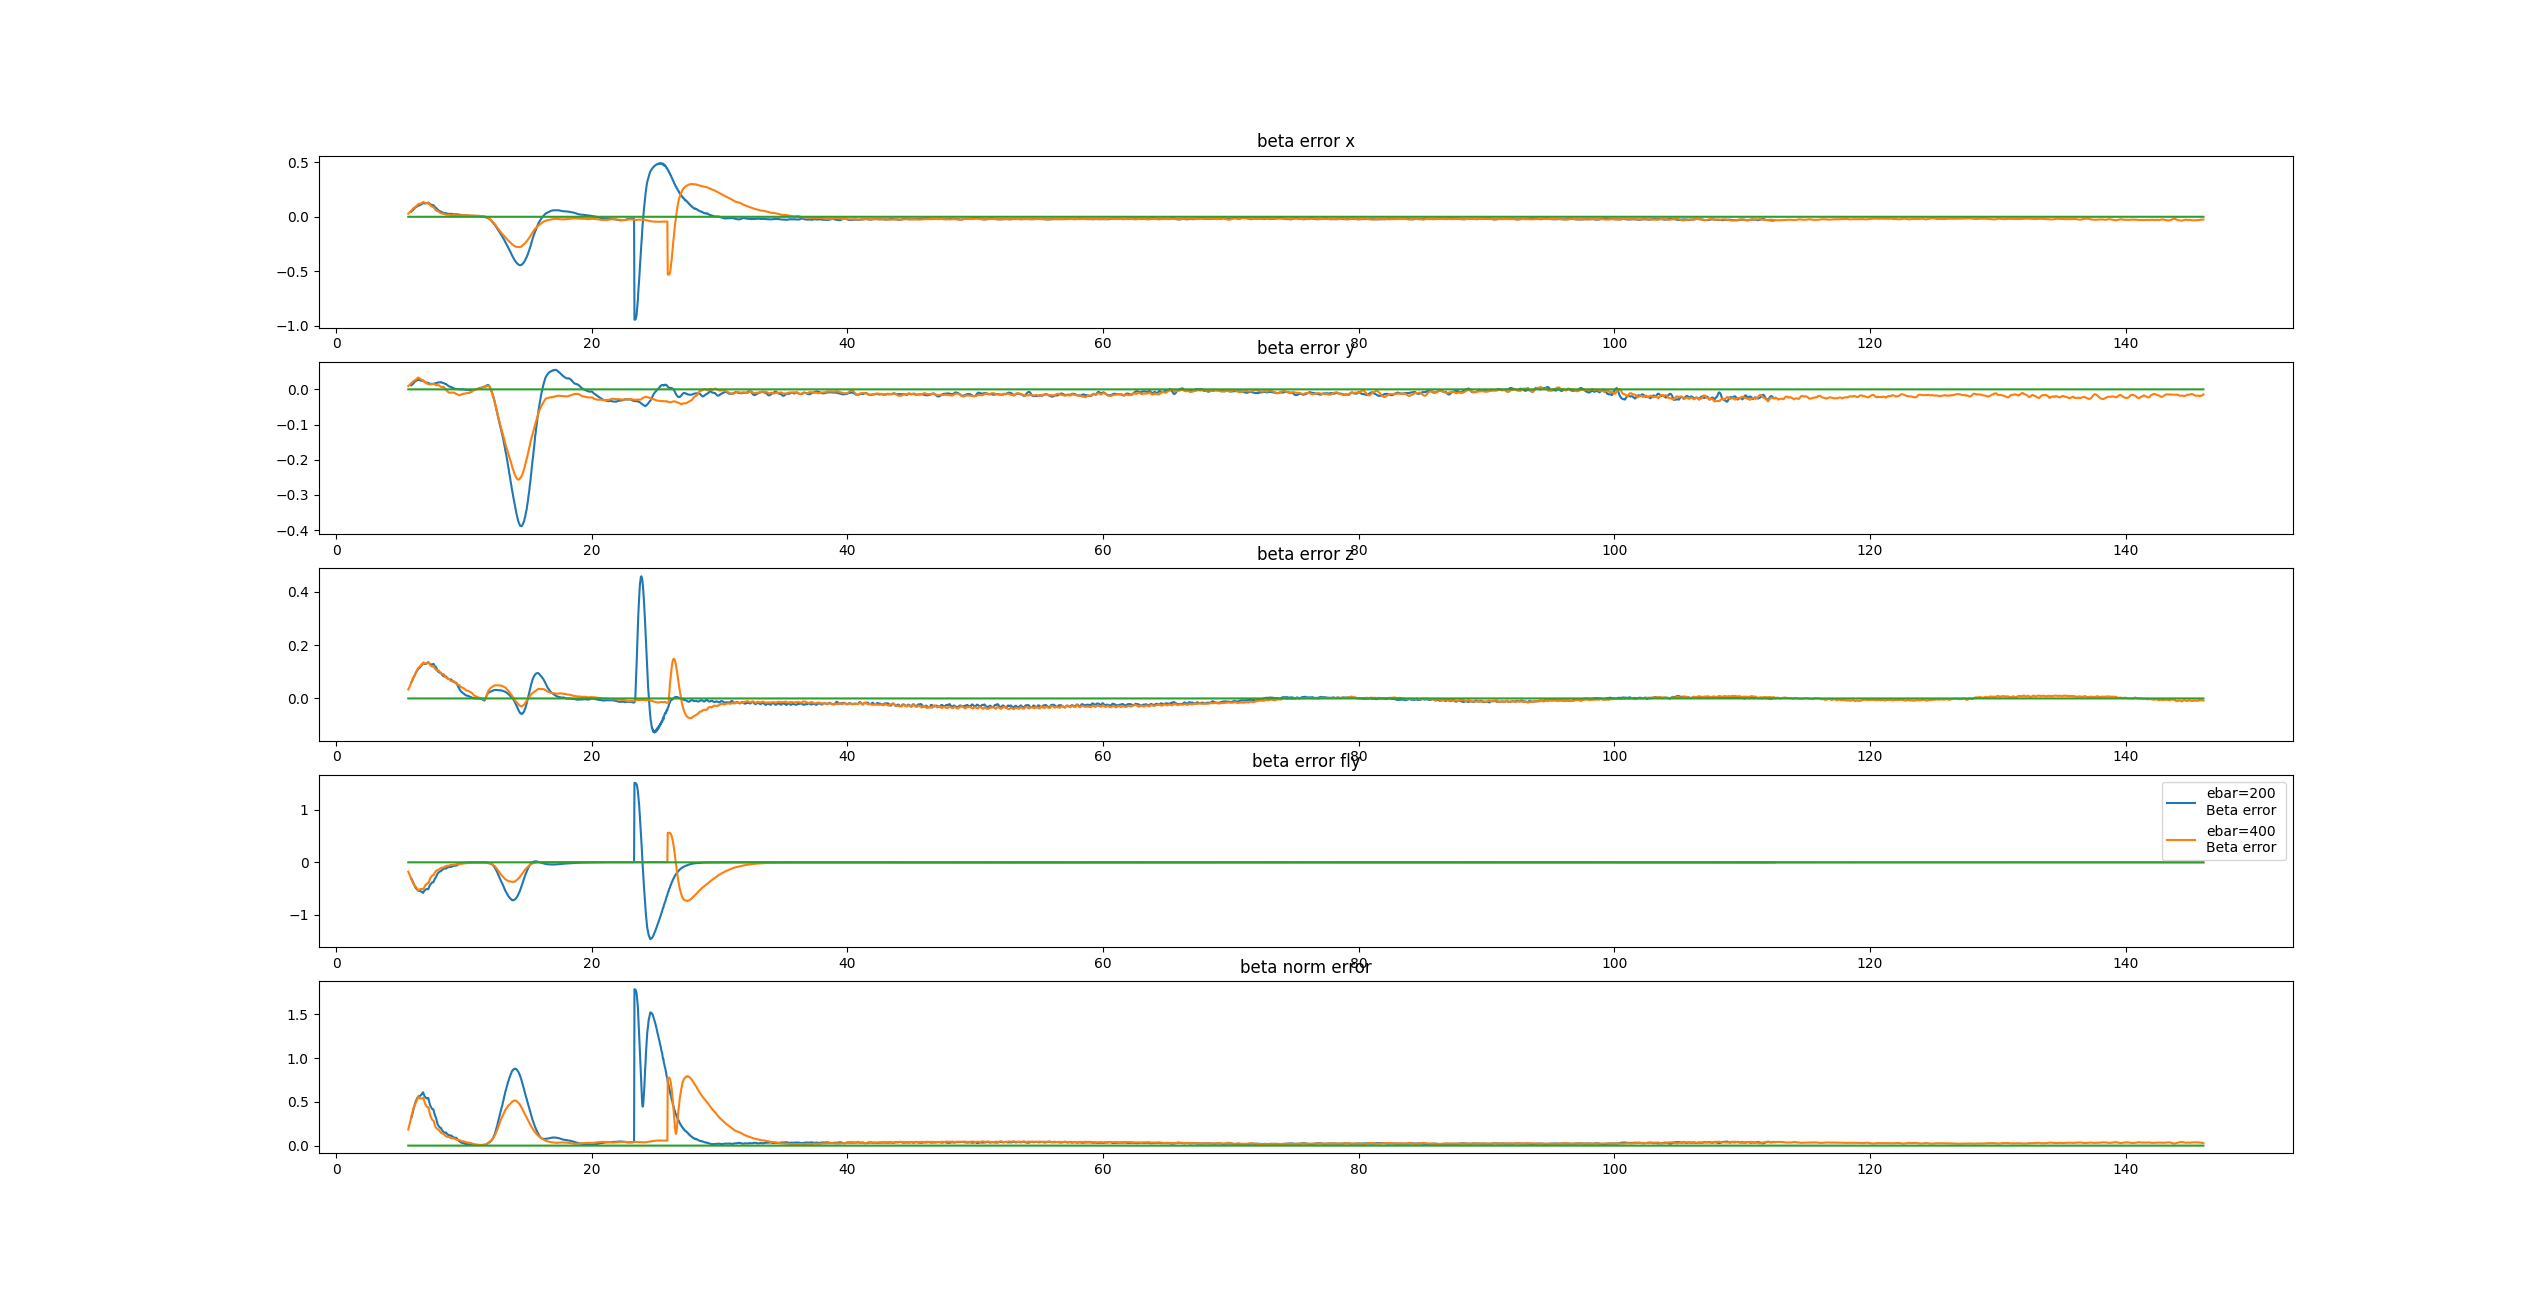
\includegraphics[width=\linewidth]{Images/gazebo_betaerror_ebar_potential.png}
   \caption{potential field $\beta$ error Gazebo - $\bar{E}$ experiment}
   \label{fig:betaerrorgazebopotentialebar}
\end{figure*}

\subsubsection{force compensation study}
Similarly to our circular field experiment, here to the drag compensation term is essential to properly follow the desired velocity field. 
\begin{figure*}[h!]
   \centering
   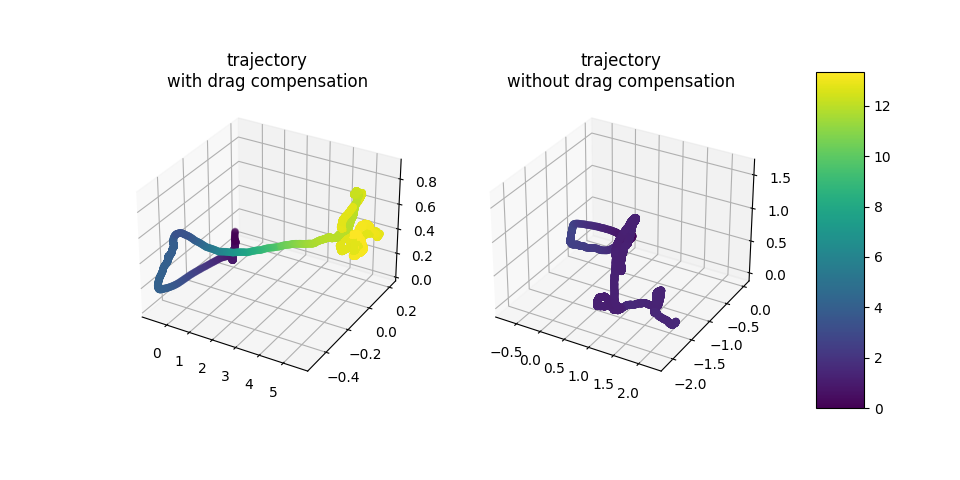
\includegraphics[width=\linewidth]{Images/gazebo_trajectory_fcomp_potential.png}
   \caption{circular field trajectory Gazebo - drag compensation experiment}
   \label{fig:trajgazebopotentialfcomp}
\end{figure*}
We can see that when no drag compensation is used, the augmented quadcopter system lose all of its mechanical energy and is unable to follow the desired potential field (see figure \ref{fig:trajgazebopotentialfcomp})
\subsection{Sensor placement experiment}
The sensor placement experiment starts in a similar way than the potential experience. 
There is an obstacle with the shape of a cylinder positioned at $(2,0)$ with a radius of $0.2$ meters and a height of $3$.
In a addition there is a wall spanning along the $\hat{y}$, $\hat{z}$ plane positioned at $x=5$
This experiment is taking place in 4 phases:
\begin{enumerate}
   \item take off following the sink field at $(0,0,0.5)$ to gain altitude, when the desired altitude was reached, we switch to the next phase 
   \item Following the sink field with sink point at $(5,0,0.5)$, this is to reach the wall. While following this field, the obstacle will be encountered by the quadcopter and the PCL node will signal to the velocity field node the new obstacle. Upon this signal, the velocity field adds a repulsive field to the current sink field. 
   \item When the wall has been reached and contact was made between the arm and the wall, the modified grasping arm plugin from gazebo will activate for 10 seconds.
   \item After the grasping arm disengage, a signal is sent to the velocity field node to update the sink field with a sink point on the floor close to the wall.
\end{enumerate}
A state machine is implemented in the velocity field node to switch and chose the right velocity field for each step. 
A \href{https://www.youtube.com/watch?v=bR4PmFp38t0}{video} of this Gazebo experiment was published to Youtube. (Please watch with subtitles)
Let us analyse the beta error and trajectory of this experiment.
We can see in figure \ref{fig:trajgazebosensor} that the flywheel energy is state when reaching the wall and increasing when contact is made. This is because of the passivity of PVFC dissipating the work of the wall inside the augmented system.
The $\beta$ error in figure \ref{fig:betaerrorgazebosensor} is spiking at each field update, the spike at $t=10s$ is due to the change from take off field to approach field (the field to reach the wall). 
The spike at $t=30s$ is due to the added cylinder repulsive field to the approach field.
The spike at $t=45s$ is due to the contact with the wall. Between $t=45s$ and $t=55s$, the $\beta$ error norm is unable to decrease because of the work from the wall on the tip of the arm. 
The small spike at $t=75s$ is due to the quad landing causing work from the floor on the quad.

\begin{figure*}[h!]
   \centering
   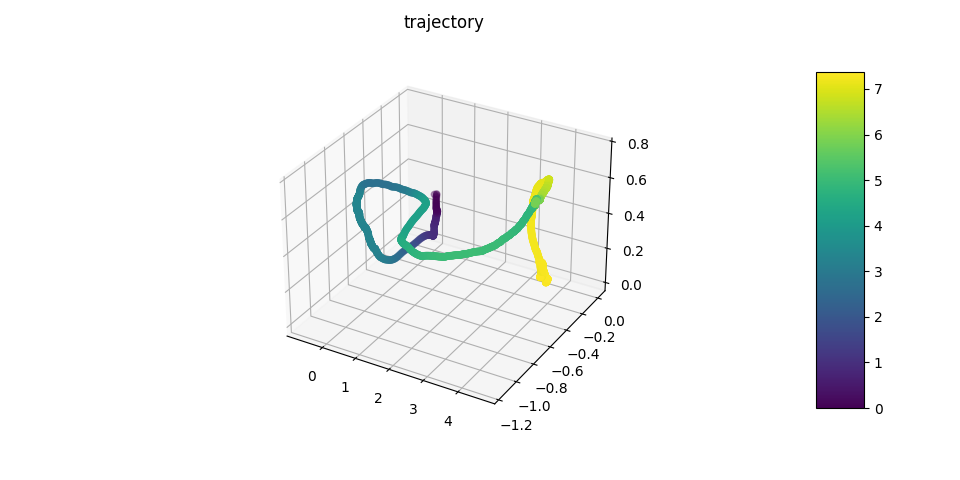
\includegraphics[width=\linewidth]{Images/gazebo_trajectory_sensor.png}
   \caption{Sensor placement trajectory Gazebo}
   \label{fig:trajgazebosensor}
\end{figure*}
\begin{figure*}[h!]
   \centering
   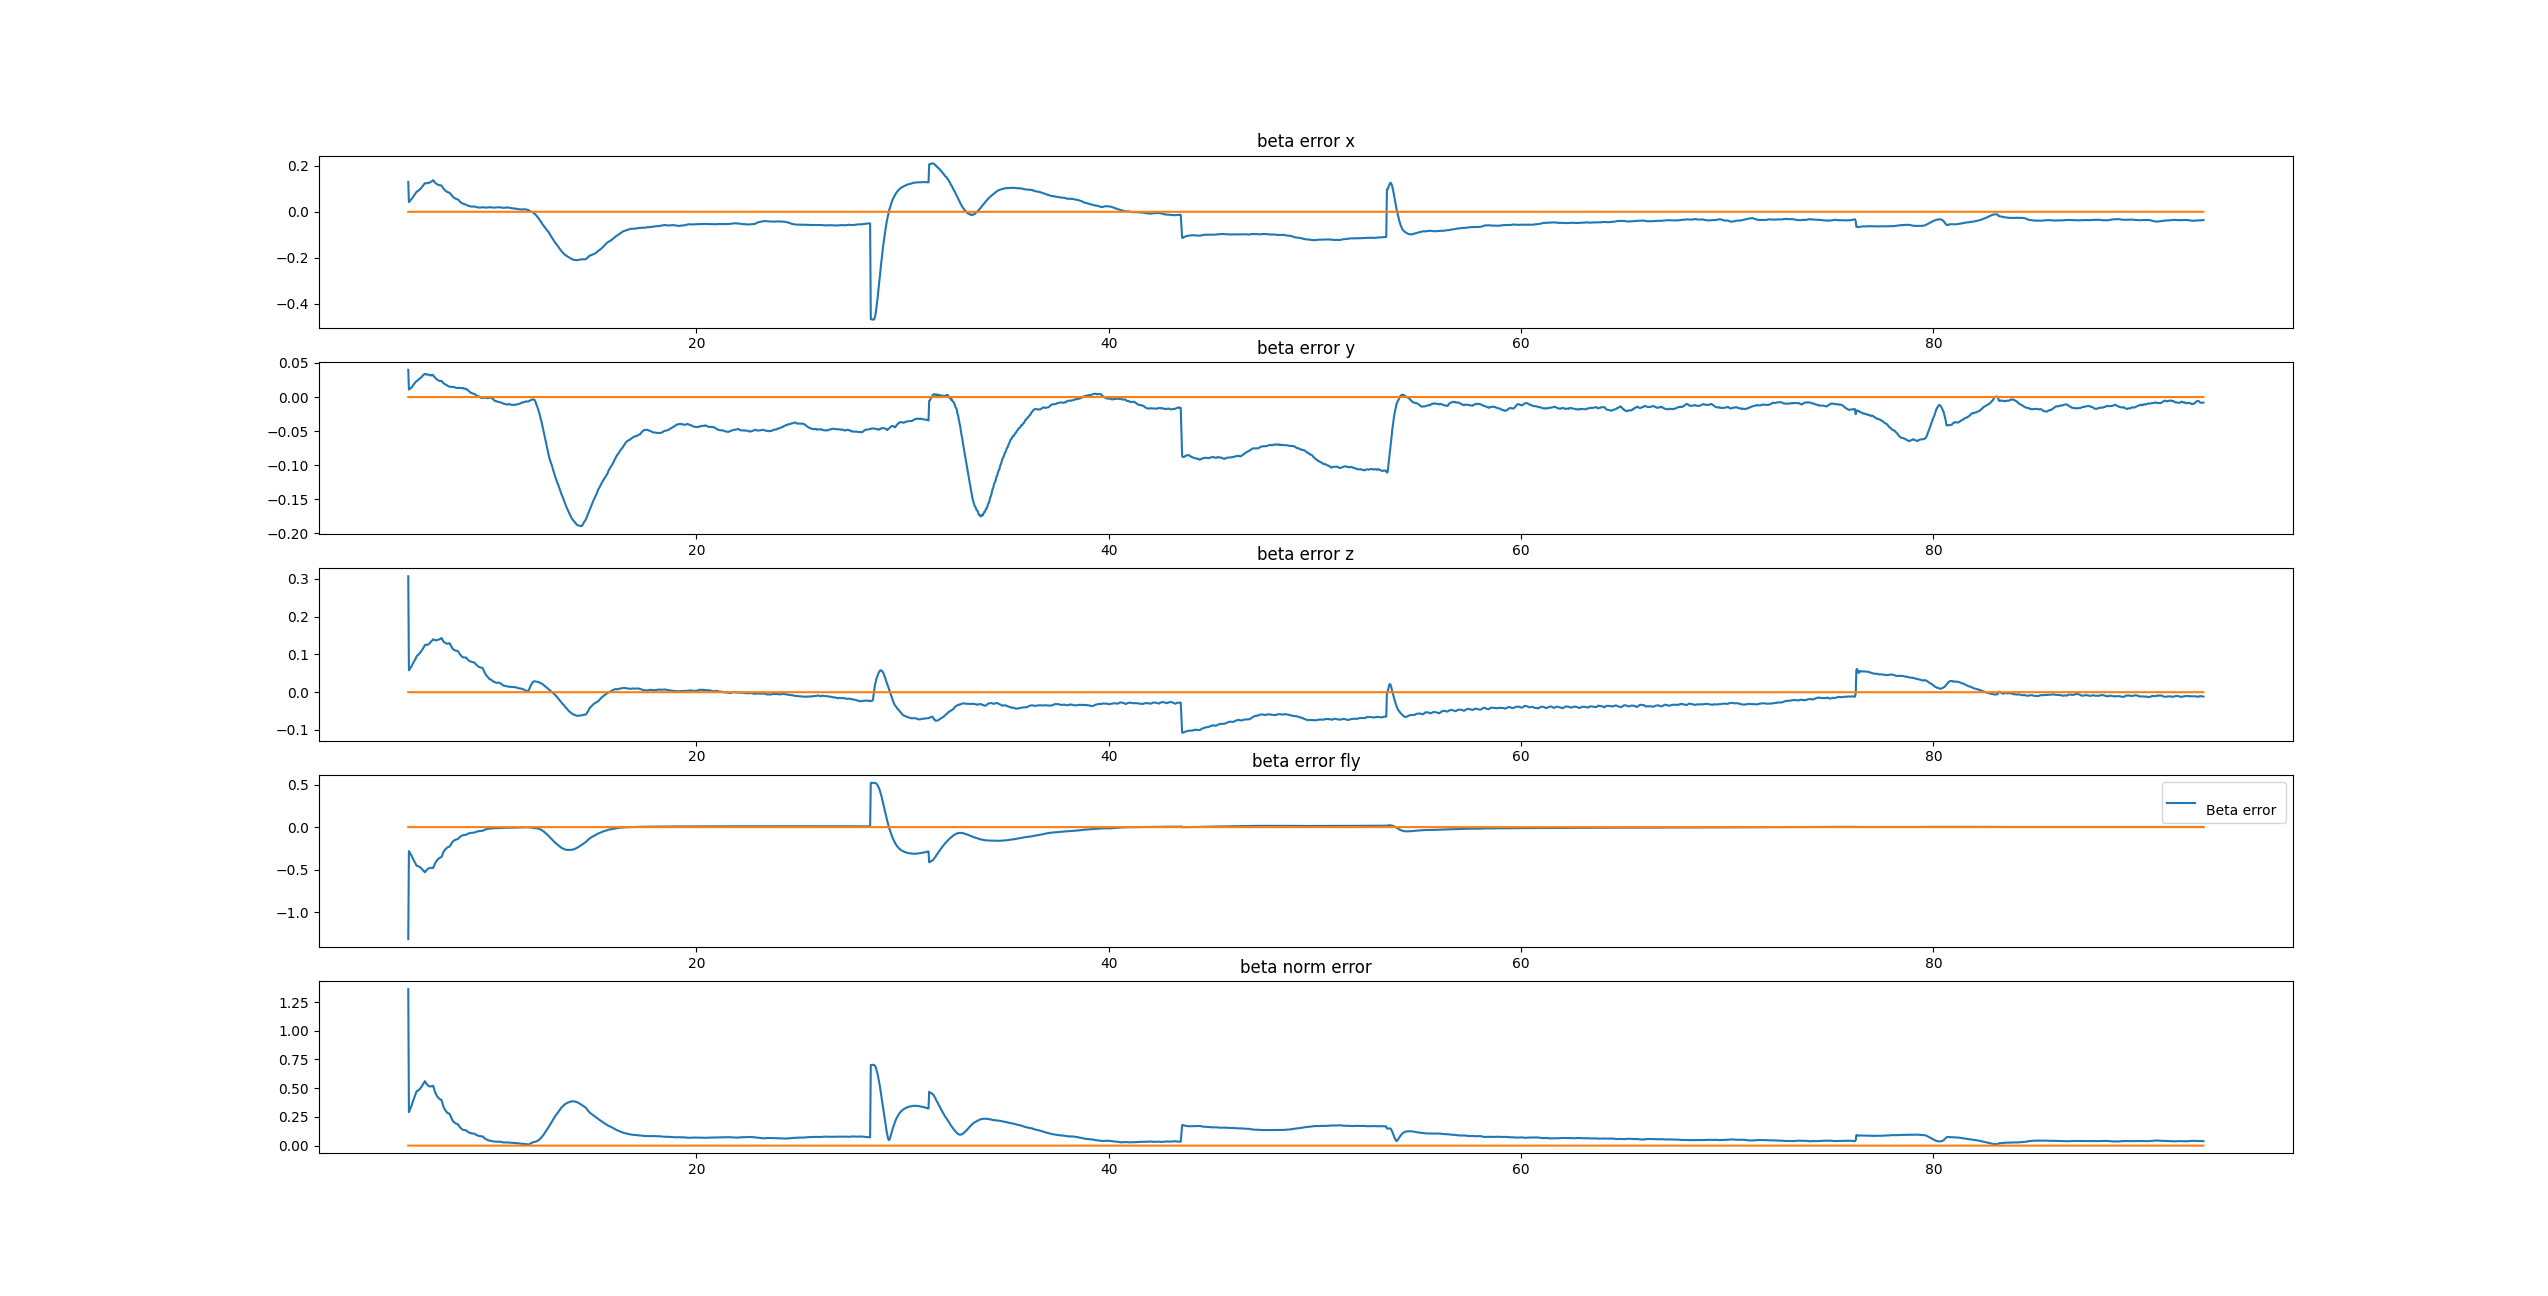
\includegraphics[width=\linewidth]{Images/gazebo_betaerror_sensor.png}
   \caption{Sensor placement $\beta$ error Gazebo}
   \label{fig:betaerrorgazebosensor}
\end{figure*}

